%%%%%%%%%%%%%%%%%%%%%%%%%%%%%%%%%%%%%%%%%%%%%%%%%%%%%%%%%%%%%%%%%%%%%%
% Lớp 11 | Hàm số lượng giác và phương trình lượng giác | Hàm số lượng giác và đồ thị
% Dạng 1D1?4-2: Tìm tập xác định
% Số câu: 122  (sinh tự động bởi tach_cau.py; từ nay thầy sửa trực tiếp file này)
%%%%%%%%%%%%%%%%%%%%%%%%%%%%%%%%%%%%%%%%%%%%%%%%%%%%%%%%%%%%%%%%%%%%%%

%%%%%%%%%%%%%%%% TRẮC NGHIỆM 4 PHƯƠNG ÁN %%%%%%%%%%%%%%%%

% nguồn: Ok_Toan11_TracNghiem_Lan2
\begin{ex}%[1D1N4-2]%[ma:1a0ffbe3]
	Tập xác  định của hàm số $y=\dfrac{1+\sin x}{\cos x}$ là
	 \choice
		{$\mathscr{D}=\mathbb{R}\setminus\left\{k\pi ,k\in\mathbb{Z}\right\}$} 
		{\True  $\mathscr{D}=\mathbb{R}\setminus\left\{\dfrac{\pi}{2}+k\pi ,k\in\mathbb{Z}\right\}$}
		{$\mathscr{D}=\mathbb{R}\setminus\left\{k2\pi  ,k\in\mathbb{Z}\right\}$}
		{$\mathscr{D}=\mathbb{R}\setminus\left\{\dfrac{\pi}{2}+k2\pi  ,k\in\mathbb{Z}\right\}$}
	\loigiai{ 
	Hàm số đã cho xác định khi $\cos x\ne  0\Leftrightarrow x\ne\dfrac{\pi}{2}+k\pi$, $k\in\mathbb{Z}$.\\
	Vậy tập xác định của hàm  số đã cho là $\mathscr{D}=\mathbb{R}\setminus\left\{\dfrac{\pi}{2}+k\pi ,k\in\mathbb{Z}\right\}$.
	} 
\end{ex}

% nguồn: Ok_Toan11_TracNghiem_Lan2
\begin{ex}%[1D1N4-2]%[ma:3ca96064]
	Tập  xác định của hàm số $y=\cot x$ là
	\choice 
		{\True $\mathscr{D}=\mathbb{R}\setminus\{k\pi  ,k\in\mathbb{Z}\}$}
		 {$\mathscr{D}=\mathbb{R}\setminus\left\{\dfrac{\pi}{2}+k2\pi ,k\in\mathbb{Z}\right\}$}
		 {$\mathscr{D}=\mathbb{R}\setminus\left\{\dfrac{\pi}{2}+k\pi ,k\in\mathbb{Z}\right\}$}
		{$\mathscr{D}=\mathbb{R}\setminus\{k2\pi ,k\in\mathbb{Z}\}$} 
	\loigiai{ 
	Hàm số đã  cho xác định khi $\sin x\ne 0\Leftrightarrow x\ne k\pi$, $k\in\mathbb{Z}$.\\
	 Vậy tập xác định của hàm số đã cho là $\mathscr{D}=\mathbb{R}\setminus\{k\pi ,k\in\mathbb{Z}\}$.
	} 
\end{ex}

% nguồn: Ok_Toan11_TracNghiem_Lan2
\begin{ex}%[1D1N4-2]%[ma:6462b9bc]
	Tập xác định của hàm số  $y=\dfrac{x^2+1}{\cos x}$ là
	\choice 
		{$\mathscr{D}=\mathbb{R}$} 
		{\True  $\mathscr{D}=\mathbb{R}\setminus\left\{\dfrac{\pi}{2}+k\pi ,k\in\mathbb{Z}\right\}$}
		{$\mathscr{D}=\mathbb{R}\setminus\{k\pi ,k\in\mathbb{Z}\}$} 
		 {$\mathscr{D}=\mathbb{R}\setminus\left\{\dfrac{k\pi}{2},k\in\mathbb{Z}\right\}$}
	 \loigiai{
	Hàm số đã cho xác  định khi $\cos x\ne 0\Leftrightarrow x\ne\dfrac{\pi}{2}+k\pi$, $K\in\mathbb{Z}$.\\
	Vậy tập xác định của hàm số đã cho là $\mathscr{D}=\mathbb{R}\setminus\left\{\dfrac{\pi}{2}+k\pi ,k\in\mathbb{Z}\right\}$. 
	 }
\end{ex}

% nguồn: Ok_Toan11_TracNghiem_Lan2
\begin{ex}%[1D1N4-2]%[ma:6be9208d]
	Tập xác định  của hàm số $y=\cot x$ là
	\choice 
		 {$\mathscr{D}=\mathbb{R}$}
		{$\mathscr{D}=\mathbb{R}\setminus \left\{k\dfrac{\pi}{2},k\in \mathbb{Z}  \right\}$}
		{$\mathscr{D}=\mathbb{R}\setminus  \left\{\pi+k\dfrac{\pi}{2},k\in \mathbb{Z}\right\}$}
		{\True $\mathscr{D}=\mathbb{R}\setminus \left\{k\pi,k\in  \mathbb{Z}\right\}$}
	 \loigiai{
		Điều kiện $\sin  x\ne 0\Leftrightarrow x\ne k\pi$, $k\in \mathbb{Z}$.\\
		Do đó, tập xác định  của hàm số $y=\cot x$ là $\mathscr{D}=\mathbb{R}\setminus \left\{k\pi,k\in \mathbb{Z} \right\}$.
	 }
\end{ex}

% nguồn: Ok_Toan11_TracNghiem_Lan2
\begin{ex}%[1D1N4-2]%[ma:b4fc5533]
	Tập xác định của hàm số $y=\dfrac{2021}{1-\cos  x}$ là
	\choice 
		{$\mathscr{D}=\mathbb{R}\setminus\left\{\dfrac{k\pi}{2} ,k\in\mathbb{Z}\right\}$} 
		{\True $\mathscr{D}=\mathbb{R}\setminus\left\{k2\pi ,k\in\mathbb{Z}\right\}$} 
		{$\mathscr{D}=\mathbb{R}\setminus\left\{\dfrac{\pi}{2}+k\pi ,k\in\mathbb{Z}\right\}$} 
		{$\mathscr{D}=\mathbb{R}\setminus\left\{k\pi ,k\in\mathbb{Z}\right\}$} 
	\loigiai{ 
	 Hàm số đã cho xác định khi $\cos x\ne 1\Leftrightarrow x\ne k2\pi$, $k\in\mathbb{Z}$.\\
	Vậy tập xác định của hàm số đã  cho là $\mathscr{D}=\mathbb{R}\setminus\left\{k2\pi ,k\in\mathbb{Z}\right\}$.
	 }
\end{ex}

% nguồn: Ok_Toan11_TracNghiem_Lan2
\begin{ex}%[1D1N4-2]%[ma:93174ca7]
	Tập xác định của hàm số  $y=\dfrac{1}{\sin x}$ là
	\choice 
		 {$\mathscr{D}=\mathbb{R}\setminus\{0\}$}
		{$\mathscr{D}=\mathbb{R}\setminus\{k2\pi  ,k\in\mathbb{Z}\}$}
		{\True  $\mathscr{D}=\mathbb{R}\setminus\{k\pi ,k\in\mathbb{Z}\}$}
		{$\mathscr{D}=\mathbb{R}\setminus\{0;\pi\}$} 
	 \loigiai{
	Hàm số đã cho xác định khi $\sin x\ne 0\Leftrightarrow x\ne k\pi$, $k\in\mathbb{Z}$.\\ 
	Vậy tập  xác định của hàm số đã cho là $\mathscr{D}=\mathbb{R}\setminus\{k\pi ,k\in\mathbb{Z}\}$.
	 }
\end{ex}

% nguồn: Ok_Toan11_TracNghiem_Lan2
\begin{ex}%[1D1N4-2]%[ma:aeac3d94]
	Tìm tập xác định $\mathscr{D}$ của hàm số $y=\dfrac{1-\sin  x}{1+\cos x}$.
	\choice 
		{$\mathscr{D}=\mathbb{R}\setminus\left\{-\dfrac{\pi}{2}+k2\pi  ,\dfrac{\pi}{2}+k2\pi ,k\in\mathbb{Z}\right\}$}
		 {$\mathscr{D}=\mathbb{R}\setminus\left\{-k\pi ,k\in\mathbb{Z}\right\}$}
		{\True $\mathscr{D}=\mathbb{R}\setminus\left\{\pi +k2\pi ,k\in\mathbb{Z}\right\}$} 
		{$\mathscr{D}=\mathbb{R}\setminus\left\{ \dfrac{\pi}{2}+k2\pi,k\in\mathbb{Z}\right\}$} 
	 \loigiai{
	Hàm số đã cho xác định khi $\cos x\ne -1\Leftrightarrow x\ne\pi  +k2\pi$, $k\in\mathbb{Z}$.\\
	Vậy tập xác định của hàm số đã cho là  $\mathscr{D}=\mathbb{R}\setminus\left\{\pi +k2\pi ,k\in\mathbb{Z}\right\}$.
	 }
\end{ex}

% nguồn: Ok_Toan11_TracNghiem_Lan2
\begin{ex}%[1D1N4-2]%[ma:6f9f57fc]
	Khẳng định nào sau đây là  đúng
	\choice 
		 {\True $\cos x\ne 0\Leftrightarrow x\ne \dfrac{\pi}{2}+k\pi$, $k\in \mathbb{Z}$}
		{$\cos x\ne 1\Leftrightarrow x\ne \dfrac{\pi}{2}+k\pi$, $k\in  \mathbb{Z}$}
		{$\cos x\ne 0\Leftrightarrow x\ne \dfrac{\pi}{2}+k2\pi$, $k\in  \mathbb{Z}$}
		{$\cos x\ne-1\Leftrightarrow  x\ne \dfrac{\pi}{2}+k2\pi$, $k\in \mathbb{Z}$}
	\loigiai{ 
		Ta có $\cos x\ne 0\Leftrightarrow x\ne \dfrac{\pi}{2}+k\pi$, $k\in \mathbb{Z}$. 
	 }
\end{ex}

% nguồn: Ok_Toan11_TracNghiem_Lan2
\begin{ex}%[1D1N4-2]%[ma:f233930d]
	Tập xác định  của hàm số $y=\dfrac{1-\sin x}{\cos x}$ là
	\choice 
		{$\mathscr{D}=\mathbb{R}\setminus\{k\pi ,k\in\mathbb{Z}\}$} 
		{$\mathscr{D}=\mathbb{R}\setminus\{k2\pi ,k\in\mathbb{Z}\}$} 
		{\True  $\mathscr{D}=\mathbb{R}\setminus\left\{\dfrac{\pi}{2}+k\pi ,k\in\mathbb{Z}\right\}$}
		 {$\mathscr{D}=\mathbb{R}\setminus\left\{-\dfrac{\pi}{2}+k2\pi ,k\in\mathbb{Z}\right\}$}
	 \loigiai{
	Hàm số đã  cho xác định khi $\cos x\ne 0\Leftrightarrow x\ne\dfrac{\pi}{2}+k\pi$, $K\in\mathbb{Z}$.\\
	Vậy  tập xác định của hàm số đã cho là $\mathscr{D}=\mathbb{R}\setminus\left\{\dfrac{\pi}{2}+k\pi ,k\in\mathbb{Z}\right\}$.
	 }
\end{ex}

% nguồn: Ok_Toan11_TracNghiem_Lan2
\begin{ex}%[1D1N4-2]%[ma:5d63cd64]
	Tập xác định của hàm số  $y=\dfrac{\sin x}{2-2\cos x}$ là
	 \choice
		{$\mathscr{D}=\mathbb{R}$} 
		{$\mathscr{D}=\mathbb{R}\setminus\left\{\dfrac{k\pi}{2} ,k\in\mathbb{Z}\right\}$} 
		 {$\mathscr{D}=\mathbb{R}\setminus\left\{\pi +\dfrac{k\pi}{2} ,k\in\mathbb{Z}\right\}$}
		{\True  $\mathscr{D}=\mathbb{R}\setminus\left\{k2\pi ,k\in\mathbb{Z}\right\}$}
	\loigiai{ 
	Hàm số đã cho xác  định khi $\cos x\ne 1\Leftrightarrow x\ne k2\pi$, $k\in\mathbb{Z}$.\\
	Vậy tập xác định của hàm  số đã cho là $\mathscr{D}=\mathbb{R}\setminus\left\{k2\pi ,k\in\mathbb{Z}\right\}$.
	} 
\end{ex}

% nguồn: Ok_Toan11_TracNghiem_Lan2
\begin{ex}%[1D1N4-2]%[ma:cdf28451]
	Tập xác định của hàm số $y=\dfrac{2\sin  x-1}{\cos x}$ là
	 \choice
		{\True $\mathscr{D}=\mathbb{R}\setminus\left\{  \dfrac{\pi}{2}+k\pi ,k\in\mathbb{Z}\right\}$}
		{$\mathscr{D}=\mathbb{R}\setminus\left\{ k\pi ,k\in\mathbb{Z}\right\}$} 
		{$\mathscr{D}=\mathbb{R}\setminus\left\{ \dfrac{k\pi}{2}  ,k\in\mathbb{Z}\right\}$}
		 {$\mathscr{D}=\mathbb{R}\setminus\left\{ k2\pi ,k\in\mathbb{Z}\right\}$}
	\loigiai{ 
	Hàm số  đã cho xác định khi $\cos x\ne 0\Leftrightarrow x\ne\dfrac{\pi}{2}+k\pi$, $K\in\mathbb{Z}$.\\
	Vậy tập xác định của  hàm số đã cho là $\mathscr{D}=\mathbb{R}\setminus\left\{\dfrac{\pi}{2}+k\pi ,k\in\mathbb{Z}\right\}$.
	 }
\end{ex}

% nguồn: Ok_Toan11_TracNghiem_Lan2
\begin{ex}%[1D1N4-2]%[ma:382aba48]
	Tập xác định của hàm số $y=2+3\tan  x$ là
	\choice 
		{$\mathscr{D}=\mathbb{R}\setminus\left\{\dfrac{\pi}{3}+k\pi ,k\in\mathbb{Z}\right\}$} 
		{$\mathscr{D}=\mathbb{R}\setminus\left\{\dfrac{\pi}{6}+k\pi ,k\in\mathbb{Z}\right\}$} 
		 {\True $\mathscr{D}=\mathbb{R}\setminus\left\{\dfrac{\pi}{2}+k\pi ,k\in\mathbb{Z}\right\}$}
		{$\mathscr{D}=\mathbb{R}\setminus\left\{\dfrac{\pi}{4}+k\pi ,k\in\mathbb{Z}\right\}$} 
	\loigiai{ 
	 Hàm số đã cho xác định khi $\cos x\ne 0\Leftrightarrow x\ne\dfrac{\pi}{2}+k\pi$, $K\in\mathbb{Z}$.\\
	Vậy tập xác định của hàm số đã cho  là $\mathscr{D}=\mathbb{R}\setminus\left\{\dfrac{\pi}{2}+k\pi ,k\in\mathbb{Z}\right\}$.
	} 
\end{ex}

% nguồn: Ok_Toan11_TracNghiem_Lan2
\begin{ex}%[1D1N4-2]%[ma:6b33242b]
	Tập xác định của hàm số $y=\dfrac{3+\sin  x}{\cos x-1}$ là
	\choice 
		{$\mathscr{D}=\mathbb{R}\setminus\left\{k\pi ,k\in\mathbb{Z}\right\}$} 
		{$\mathscr{D}=\mathbb{R}\setminus\left\{\dfrac{\pi}{2}+ k\pi  ,k\in\mathbb{Z}\right\}$}
		 {$\mathscr{D}=\mathbb{R}\setminus\left\{ \dfrac{\pi}{2}+k2\pi ,k\in\mathbb{Z}\right\}$}
		{\True  $\mathscr{D}=\mathbb{R}\setminus\left\{ k2\pi ,k\in\mathbb{Z}\right\}$}
	\loigiai{ 
	Hàm số đã cho xác định khi $\cos x\ne 1\Leftrightarrow x\ne k2\pi$, $k\in\mathbb{Z}$.\\ 
	Vậy tập xác định  của hàm số đã cho là $\mathscr{D}=\mathbb{R}\setminus\left\{k2\pi ,k\in\mathbb{Z}\right\}$.
	} 
\end{ex}

% nguồn: Ok_Toan11_TracNghiem_Lan2
\begin{ex}%[1D1N4-2]%[ma:f015586c]
	Tập xác  định của hàm số $y=\dfrac{2\sin x+1}{1-\cos x}$ là
	\choice 
		{\True $\mathscr{D}=\mathbb{R}\setminus\left\{k2\pi  ,k\in\mathbb{Z}\right\}$}
		 {$\mathscr{D}=\mathbb{R}\setminus\left\{\pi +k2\pi ,k\in\mathbb{Z}\right\}$}
		{$\mathscr{D}=\mathbb{R}\setminus\left\{\dfrac{\pi}{2}+k\pi ,k\in\mathbb{Z}\right\}$} 
		{$\mathscr{D}=\mathbb{R}\setminus\left\{\dfrac{\pi}{2}+k2\pi  ,k\in\mathbb{Z}\right\}$}
	\loigiai{ 
	Hàm số đã cho xác định khi $\cos x\ne  1\Leftrightarrow x\ne k2\pi$, $k\in\mathbb{Z}$.\\
	Vậy tập xác  định của hàm số đã cho là $\mathscr{D}=\mathbb{R}\setminus\left\{k2\pi ,k\in\mathbb{Z}\right\}$.
	 }
\end{ex}

% nguồn: Ok_Toan11_TracNghiem_Lan2
\begin{ex}%[1D1N4-2]%[ma:d513e56b]
	Tập xác định  của hàm số $y=\tan x$ là
	 \choice
		{$\mathscr{D}=\mathbb{R}\setminus\left\{k2\pi  ,k\in\mathbb{Z}\right\}$}
		{$\mathscr{D}=\mathbb{R}\setminus\left\{\dfrac{\pi}{2}+k2\pi  ,k\in\mathbb{Z}\right\}$}
		{\True $\mathscr{D}=\mathbb{R}\setminus\left\{\dfrac{\pi}{2}+k\pi ,k\in\mathbb{Z}\right\}$} 
		 {$\mathscr{D}=\mathbb{R}\setminus\{k\pi ,k\in\mathbb{Z}\}$}
	 \loigiai{
	Hàm số đã cho xác định khi $\cos x\ne  0\Leftrightarrow x\ne\dfrac{\pi}{2}+k\pi$, $K\in\mathbb{Z}$.\\
	Vậy tập xác  định của hàm số đã cho là $\mathscr{D}=\mathbb{R}\setminus\left\{\dfrac{\pi}{2}+k\pi ,k\in\mathbb{Z}\right\}$.
	} 
\end{ex}

% nguồn: Ok_Toan11_TracNghiem_Lan2
\begin{ex}%[1D1N4-2]%[ma:032eff85]
	Tập xác định của hàm số $y=\sin x$  là
	\choice 
		{$[-1;1]$} 
		 {$(-1;1)$}
		{$(0;+\infty)$} 
		{\True $\mathbb{R}$} 
	 \loigiai{
	Hàm số $y=\sin x$ có  tập xác định là $\mathscr{D}=\mathbb{R}$.
	 }
\end{ex}

% nguồn: Ok_Toan11_TracNghiem_Lan2
\begin{ex}%[1D1N4-2]%[ma:7b6be57d]
	Tập xác  định của hàm số $y=\dfrac{1-\cos x}{\sin x}$ là
	 \choice
		{\True  $\mathscr{D}=\mathbb{R}\setminus\left\{k\pi ,k\in\mathbb{Z}\right\}$}
		 {$\mathscr{D}=\mathbb{R}\setminus\left\{\dfrac{\pi}{2}+k\pi ,k\in\mathbb{Z}\right\}$}
		 {$\mathscr{D}=\mathbb{R}\setminus\left\{k2\pi ,k\in\mathbb{Z}\right\}$}
		{$\mathscr{D}=\mathbb{R}\setminus\left\{\dfrac{\pi}{2}+k2\pi ,k\in\mathbb{Z}\right\}$} 
	 \loigiai{
	Hàm số  đã cho xác định khi $\sin x\ne 0\Leftrightarrow x\ne k\pi$, $k\in\mathbb{Z}$.\\
	Vậy tập  xác định của hàm số đã cho là $\mathscr{D}=\mathbb{R}\setminus\{k\pi ,k\in\mathbb{Z}\}$.
	 }
\end{ex}

% nguồn: Ok_Toan11_TracNghiem_Lan2
\begin{ex}%[1D1N4-2]%[ma:01594f1a]
	Hàm số $y=\cot x$ có  tập xác định là
	 \choice
		 {\True $\mathbb{R}\setminus \left\{k\pi,k\in \mathbb{Z}\right\}$}
		{$\mathbb{R}\setminus  \left\{k2\pi,k\in \mathbb{Z}\right\}$}
		{$\mathbb{R}\setminus \left\{\dfrac{\pi}{2}+k\pi,k\in \mathbb{Z}\right\}$} 
		{$\mathbb{R}\setminus \left\{\dfrac{\pi}{2}+k2\pi,k\in \mathbb{Z}\right\}$} 
	 \loigiai{
		Điều kiện xác định $\sin x\ne 0\Leftrightarrow  x\ne k\pi \left(k\in \mathbb{Z}\right)$.\\
		Tập  xác định $\mathscr{D}=\mathbb{R}\setminus \left\{k\pi,k\in \mathbb{Z}\right\}$.
	} 
\end{ex}

% nguồn: Ok_Toan11_TracNghiem_Lan2
\begin{ex}%[1D1N4-2]%[ma:f33ab26b]
	Điều kiện xác  định của hàm số $y=\dfrac{2021-\cos x}{\sin x}$ là
	 \choice
		{$x\ne\dfrac{\pi}{2}+k\pi ,k\in\mathbb{Z}$} 
		{\True $x\ne k\pi  ,k\in\mathbb{Z}$}
		{$x\ne  k2\pi ,k\in\mathbb{Z}$}
		 {$x\ne\dfrac{k\pi}{2},k\in\mathbb{Z}$}
	 \loigiai{
	Hàm số đã cho xác định khi $\sin x\ne 0\Leftrightarrow x\ne  k\pi$, $k\in\mathbb{Z}$.
	} 
\end{ex}

% nguồn: Ok_Toan11_TracNghiem_Lan2
\begin{ex}%[1D1N4-2]%[ma:1a4b4ced]
	Khẳng định nào sau đây  là đúng?
	 \choice
		{\True Hàm số  $y=\cos x$ có tập xác định là $\mathbb{R}$}
		{Hàm số $y=\tan x$ có tập  xác định là $\mathbb{R}$}
		{Hàm số $y=\cot x$ có tập xác định  là $\mathbb{R}$}
		{Các  hàm số lượng giác có tập xác định là $\mathbb{R}$}
	\loigiai{ 
		Hàm số $y=\cos x$ có tập xác định  là $\mathbb{R}$.
	 }
\end{ex}

% nguồn: Ok_TracNghiemLop11_Lan1
\begin{ex}%[1D1N4-2]%[ma:9fd51f40]
	Tìm tập  xác định của hàm số $y=\dfrac{1-\sin x}{\cos x}$
	\choice 
		{\True $x\ne \dfrac{\pi }{2}+k\pi,  k\in \mathbb{Z} $}
		{$x\ne -\dfrac{\pi }{2}+k2\pi, k\in \mathbb{Z} $ } 
		{$x\ne \dfrac{\pi }{2}+k2\pi,  k\in \mathbb{Z} $}
		{$x\ne k\pi, k\in \mathbb{Z}  $}
	 \loigiai{
	Hàm số $y=\dfrac{1-\sin x}{\cos x}$  xác định khi $\cos x\ne 0\Leftrightarrow x\ne \dfrac{\pi }{2}+k\pi $.}
\end{ex}

% nguồn: Ok_TracNghiemLop11_Lan1
\begin{ex}%[1D1N4-2]%[ma:b03fabee]
	Tập xác định của hàm số $y=\tan x$ là 
	 \choice
		 {$\mathbb{R}$}
		 {$\mathbb{R}\setminus \left\{\dfrac{\pi}{2}+k2\pi ,k\in \mathbb{Z} \right\}$}
		{\True $\mathbb{R}\setminus  \left\{\dfrac{\pi}{2}+k\pi ,k\in \mathbb{Z} \right\}$}
		{$\mathbb{R}\setminus \left\{k\pi  ,k\in \mathbb{Z} \right\}$}
	 \loigiai{
		Hàm số trên  xác định khi $\cos x\ne 0
		 \Leftrightarrow x\ne \dfrac{\pi}{2}+k\pi $.\\
		Vậy tập xác định của hàm số là $\mathscr{D}=\mathbb{R}\setminus \left\{\dfrac{\pi}{2}+k\pi ,k\in \mathbb{Z}  \right\}$.
	} 
\end{ex}

% nguồn: Ok_TracNghiemLop11_Lan1
\begin{ex}%[1D1N4-2]%[ma:81bde023]
	 Điều kiện xác định của hàm số $y=\dfrac{1-2 \sin x}{\cos x}$ là
	\choice 
		{$x \neq \dfrac{\pi}{2}+k 2 \pi,  k \in \mathbb{Z}$}
		{\True $x \neq \dfrac{\pi}{2}+k \pi, k \in  \mathbb{Z}$}
		{$x \neq  k{2}\pi, k \in \mathbb{Z}$}
		{$x \neq k \pi,  k \in \mathbb{Z}$}
	 \loigiai{
		Để hàm số $y=\dfrac{1-2  \sin x}{\cos x}$ xác định thì
		$$ 
		\cos x \ne  0
		 \Leftrightarrow
		x \ne \dfrac{\pi}{2} + k\pi, \,  (k \in \mathbb{Z}).
		 $$
	 }
\end{ex}

% nguồn: Ok_TracNghiemLop11_Lan1
\begin{ex}%[1D1N4-2]%[ma:11f081e6]
	Tập xác định của hàm số $y=\dfrac{2\sin  x+1}{1-\cos x}$ là
	 \choice
		{\True $\mathscr{D} = \mathbb{R}\backslash\{k2\pi, k\in \mathbb{Z}\}  $}
		{$\mathscr{D}  = \mathbb{R}\backslash\{ k\pi, k\in \mathbb{Z} \} $}
		 {$\mathscr{D} = \mathbb{R}\backslash\left\{ \dfrac{\pi }{2}+k\pi, k\in \mathbb{Z} \right\} $}
		{$\mathscr{D} = \mathbb{R}\backslash\left\{ \dfrac{\pi }{2}+k2\pi,  k\in \mathbb{Z} \right\} $}
	\loigiai{ 
	Hàm số xác định khi $1-\cos x\ne 0\Leftrightarrow x\ne k2\pi, k\in \mathbb{Z}$.} 
\end{ex}

% nguồn: Ok_TracNghiemLop11_Lan1
\begin{ex}%[1D1N4-2]%[ma:96fe302d]
	Tìm tập xác định $\mathscr{D}$ của hàm  số $y=\dfrac{2019}{\sin x}$
	 \choice
		{$\mathscr{D}=\mathbb{R}\backslash \left\{ \dfrac{\pi  }{2}+k\pi ,k\in \mathbb{Z} \right\}$}
		{$\mathscr{D}=\mathbb{R}$} 
		{$\mathscr{D}=\mathbb{R}\backslash  \left\{ 0 \right\}$ }
		{\True $\mathscr{D}=\mathbb{R}\backslash \left\{  k\pi ,k\in \mathbb{Z} \right\}$}
	 \loigiai{
		Hàm số xác định khi $\sin x\ne 0\Leftrightarrow x\ne k\pi \left( k\in \mathbb{Z} \right)$.\\ 
	Tập xác  định $\mathscr{D}=\mathbb{R}\backslash \left\{ k\pi ,k\in \mathbb{Z} \right\}$.}
\end{ex}

% nguồn: Ok_TracNghiemLop11_Lan1
\begin{ex}%[1D1N4-2]%[ma:a48a500b]
	Tập xác định của hàm số \( y = \tan 2x \) là 
	 \choice
		{\( \mathscr{D} =  \mathbb{R}\backslash \left\{ \dfrac{\pi }{4}+k\pi ,k\in \mathbb{Z} \right\} \)}
		{\True \( \mathscr{D} = \mathbb{R}\backslash \left\{ \dfrac{\pi }{4}+k\dfrac{\pi }{2},k\in  \mathbb{Z} \right\} \)}
		{\( \mathscr{D} = \mathbb{R}\backslash  \left\{ k\dfrac{\pi }{2},k\in \mathbb{Z} \right\} \)}
		{\( \mathscr{D} = \mathbb{R}\backslash \left\{ \dfrac{\pi }{2}+k\pi ,k\in  \mathbb{Z} \right\} \)}
	\loigiai{ 
		Điều kiện \(  \cos 2x \neq 0 \Leftrightarrow 2x \neq \dfrac{\pi }{2}+k\pi \Leftrightarrow x \neq \dfrac{\pi }{4}+k\dfrac{\pi }{2}, k \in \mathbb{Z} \).\\
	Vậy tập xác định là \( \mathscr{D} = \mathbb{R}\backslash \left\{ \dfrac{\pi }{4}+k\dfrac{\pi }{2},k\in \mathbb{Z} \right\} \).} 
\end{ex}

% nguồn: Ok_TracNghiemLop11_Lan1
\begin{ex}%[1D1N4-2]%[ma:35148819]
	Trong các hàm số sau,  hàm số nào có tập xác định là $\mathbb{R}$?
	\choice 
		 {$y=2-\tan x$}
		{\True $y=x^2-3\cos x$} 
		 {$y=x+\cot x$}
		{$y=\dfrac{1}{\sin^2x}$} 
	\loigiai{ 
		Hàm số $y=x^2-3\cos x$  có tập xác định là $\mathscr{D}=\mathbb{R}$.
	 }
\end{ex}

% nguồn: Ok_Toan11_TracNghiem_Lan2
\begin{ex}%[1D1H4-2]%[ma:c2e27c7d]
	Tập xác định của  hàm số $ y=\dfrac{3\cot x}{2\sin x-4}$ là
	 \choice
		{$\mathbb{R}\setminus\{2+k2\pi,\,\pi-2+k2\pi, k\in \mathbb{Z}\}$} 
		 {$\mathbb{R}$}
		{$\mathbb{R}\setminus \{\pm 2+k2\pi, k\in  \mathbb{Z}\}$}
		{\True  $\mathbb{R}\setminus \{k\pi, k\in \mathbb{Z}\}$}
	 \loigiai{
		Ta có $2\sin x-4\ne 0,\,\forall x\in  \mathbb{R}$,\\
		Nên hàm số xác định khi $\cot x$ xác định $\Leftrightarrow \sin  x\ne 0\Leftrightarrow x\ne k\pi, k\in \mathbb{Z}$.\\
	Vậy tập xác định của hàm số là $\mathbb{R}\setminus \{k\pi, k\in \mathbb{Z}\}$.} 
\end{ex}

% nguồn: Ok_Toan11_TracNghiem_Lan2
\begin{ex}%[1D1H4-2]%[ma:1c5c7e4d]
	Tìm tập xác định $\mathscr{D}$ của hàm  số $ y=\dfrac{1}{\sqrt{1+\sin x}}$.
	\choice 
		{$\mathscr{D}=\mathbb{R}\setminus \{k2\pi, k\in\mathbb{Z}\}$} 
		{$\mathscr{D}=\mathbb{R}\setminus \{\pi+k2\pi,  k\in\mathbb{Z}\}$}
		{$\mathscr{D}=\mathbb{R}\setminus \left\{\dfrac{\pi}{2}+k2\pi,\,  k\in\mathbb{Z}\right\}$}
		{\True $\mathscr{D}=\mathbb{R}\setminus\left\{\dfrac{-\pi}{2}+k2\pi,\, k\in\mathbb{Z}\right\}$} 
	 \loigiai{
		Điều kiện xác định của hàm số  là $1+\sin x>0$.\\
		Mà $1+\sin x\ge 0,\forall  x\in\mathbb{R}$.\\
		Nên $1+\sin x\ne  0\Leftrightarrow\sin x\ne-1\Leftrightarrow x\ne-\dfrac{\pi}{2}+k2\pi,\,k\in\mathbb{Z}$.\\
	Vậy tập xác định của hàm số đã cho là $\mathscr{D}=\mathbb{R}\setminus\left\{\dfrac{-\pi}{2}+k2\pi,\, k\in\mathbb{Z}\right\}$.} 
\end{ex}

% nguồn: Ok_Toan11_TracNghiem_Lan2
\begin{ex}%[1D1H4-2]%[ma:77df897f]
	Tập xác định $\mathscr{D}$ của hàm  số $y=\dfrac{5\sin x}{\cos x-3}$ là
	\choice 
		{$\mathscr{D}=(3;+\infty)$} 
		{$\mathscr{D}=\mathbb{R}\setminus\{3\}$} 
		 {$\mathscr{D}=(-\infty;3)$}
		{\True  $\mathscr{D}=\mathbb{R}$}
	\loigiai{ 
	Hàm số đã cho  xác định khi $\cos x\ne 3$.\\
	Mà $\cos x\in [-1;1]$ với mọi $x\in\mathbb{R}$.\\ 
	Vậy tập  xác định của hàm số đã cho là $\mathscr{D}=\mathbb{R}$.
	} 
\end{ex}

% nguồn: Ok_Toan11_TracNghiem_Lan2
\begin{ex}%[1D1H4-2]%[ma:a2dcab2c]
	Tập xác  định của hàm số $y=\tan 2x$ là
	\choice 
		{$\mathscr{D}=\mathbb{R}\setminus\left\{\dfrac{\pi}{4}+k\pi ,  k\in\mathbb{Z}\right\}$}
		{\True $\mathscr{D}=\mathbb{R}\setminus\left\{\dfrac{\pi}{4}+\dfrac{k\pi}{2},k\in\mathbb{Z}\right\}$} 
		 {$\mathscr{D}=\mathbb{R}\setminus\left\{\dfrac{\pi}{2}+k2\pi ,k\in\mathbb{Z}\right\}$}
		 {$\mathscr{D}=\mathbb{R}\setminus\left\{\dfrac{\pi}{2}+k\pi ,k\in\mathbb{Z}\right\}$}
	 \loigiai{
	Hàm số đã cho xác định  khi $\cos 2x\ne 0\Leftrightarrow 2x\ne\dfrac{\pi}{2}+k\pi\Leftrightarrow x\ne\dfrac{\pi}{4}+\dfrac{k\pi}{2}$, $k\in\mathbb{Z}$.\\
	 Vậy tập xác định của hàm số đã cho là $\mathscr{D}=\mathbb{R}\setminus\left\{\dfrac{\pi}{4}+\dfrac{k\pi}{2},k\in\mathbb{Z}\right\}$.
	 }
\end{ex}

% nguồn: Ok_Toan11_TracNghiem_Lan2
\begin{ex}%[1D1H4-2]%[ma:92009393]
	Tìm tập xác định của hàm số $y=\dfrac{\sin x}{1-2\cos  x}$.
	\choice 
		{\True $\mathscr{D}=\mathbb{R}\setminus\left\{  \pm\dfrac{\pi}{3}+k2\pi ,k\in\mathbb{Z} \right\} $ }
		 {$\mathscr{D}=\mathbb{R}\setminus\left\{ \dfrac{1}{2}\right\}$}
		{$\mathscr{D}=\mathbb{R}$} 
		{$\mathscr{D}=\mathbb{R}\setminus\left\{ \dfrac{\pi}{3}+k2\pi  ,k\in\mathbb{Z}\right\}$}
	\loigiai{ 
	Hàm số đã cho xác định khi $\cos x\ne\dfrac{1}{2}\Leftrightarrow x\ne\pm\dfrac{\pi}{3}+k2\pi$, $k\in\mathbb{Z}$.\\ 
	Vậy tập xác định của hàm số đã cho là $\mathscr{D}=\mathbb{R}\setminus\left\{ \pm\dfrac{\pi}{3}+k2\pi ,k\in\mathbb{Z}  \right\} $.
	} 
\end{ex}

% nguồn: Ok_Toan11_TracNghiem_Lan2
\begin{ex}%[1D1H4-2]%[ma:f44f4494]
	Tìm tập xác  định $\mathscr{D}$ của hàm số $y=\dfrac{2025}{\sin x}$.
	 \choice
		{$\mathscr{D}=\mathbb{R}$} 
		{$\mathscr{D}=\mathbb{R}\setminus \{0\}$} 
		{$\mathscr{D}=\mathbb{R}\setminus \left\{\dfrac{\pi}{2}+k\pi,  k\in \mathbb{Z}\right\}$}
		{\True  $\mathscr{D}=\mathbb{R}\setminus \left\{k\pi, k\in \mathbb{Z}\right\}$}
	 \loigiai{
		Điều kiện xác định của hàm số là $\sin x\ne  0\Leftrightarrow x\ne k\pi$, $ k\in \mathbb{Z}$.\\
		Vậy tập xác định của hàm số là $\mathscr{D}=\mathbb{R}\setminus \left\{k\pi, k\in \mathbb{Z}\right\}$. 
	 }
\end{ex}

% nguồn: Ok_Toan11_TracNghiem_Lan2
\begin{ex}%[1D1H4-2]%[ma:52f035ef]
	 Hàm số $ y=\dfrac{1}{\sin 2x\cos 2x}$ có tập xác định là
	\choice 
		 {$\mathscr{D}=\mathbb{R}\setminus\left\{\dfrac{\pi}{4}+\dfrac{k\pi}{2}\big|k\in\mathbb{Z}\right\}$}
		{\True  $\mathscr{D}=\mathbb{R}\setminus\left\{\dfrac{k\pi}{4}\big|k\in\mathbb{Z}\right\}$}
		{$\mathscr{D}=\mathbb{R}\setminus\left\{  k\pi \big|k\in\mathbb{Z}\right\}$}
		 {$\mathscr{D}=\mathbb{R}\setminus\left\{\dfrac{k\pi}{2}\big|k\in\mathbb{Z}\right\}$}
	 \loigiai{
		Điều kiện xác định của hàm số là $\sin 2x\cos 2x\ne 0 \Leftrightarrow\sin 4x\ne 0  \Leftrightarrow 4x\ne k\pi \Leftrightarrow x\ne\dfrac{k\pi}{4} (k\in\mathbb{Z})$.\\
	Vậy tập xác định $\mathscr{D}=\mathbb{R}\setminus\left\{\dfrac{k\pi}{4}\big|k\in\mathbb{Z}\right\}$.} 
\end{ex}

% nguồn: Ok_Toan11_TracNghiem_Lan2
\begin{ex}%[1D1H4-2]%[ma:819c6572]
	Tập xác định của  hàm số $y=\tan \left(2x+\dfrac{\pi}{3} \right)$ là
	 \choice
		{$\mathbb{R}\setminus  \left\{\dfrac{\pi}{6}+k\pi,k\in \mathbb{Z}\right\}$}
		{$\mathbb{R}\setminus  \left\{\dfrac{\pi}{2}+k\pi,k\in \mathbb{Z}\right\}$}
		{$\mathbb{R}\setminus \left\{\dfrac{\pi}{12}+k\pi,k\in \mathbb{Z}\right\}$} 
		 {\True $\mathbb{R}\setminus \left\{\dfrac{\pi}{12}+\dfrac{k\pi}{2},k\in \mathbb{Z}\right\}$}
	 \loigiai{
		Điều kiện xác định \allowdisplaybreaks 
		\begin{eqnarray*}
			\cos\left(2x+\dfrac{\pi}{3} \right)\ne 0&\Leftrightarrow& 2x+\dfrac{\pi}{3} \ne \dfrac{\pi}{2}+k\pi\\ 
			&\Leftrightarrow&x\ne  \dfrac{\pi}{12}+\dfrac{k\pi}{2}, k\in \mathbb{Z}.
		\end{eqnarray*}
		Vậy $\mathscr{D}=\mathbb{R}\setminus \left\{\dfrac{\pi}{12}+\dfrac{k\pi}{2},k\in \mathbb{Z}\right\}$. 
	 }
\end{ex}

% nguồn: Ok_Toan11_TracNghiem_Lan2
\begin{ex}%[1D1H4-2]%[ma:05b31d27]
	Điều kiện xác định của hàm số $y=\dfrac{2\sin  ^2x+1}{1+\cos x}$ là
	 \choice
		{$x\ne k\pi$, $ k\in  \mathbb{Z}$}
		 {\True $x\ne \pi-k2\pi$, $ k\in \mathbb{Z}$}
		{$x\ne k2\pi$, $ k\in  \mathbb{Z}$}
		{$x\ne \dfrac{\pi}{2}+k2\pi$, $  k\in \mathbb{Z}$}
	 \loigiai{
		Hàm số xác định khi $1+\cos x\ne 0\Leftrightarrow x\ne \pi-k2\pi$, $  k\in \mathbb{Z}$.
	} 
\end{ex}

% nguồn: Ok_Toan11_TracNghiem_Lan2
\begin{ex}%[1D1H4-2]%[ma:0447eb77]
	Tìm tập xác định của hàm số $y=\dfrac{1}{\sin  2x-1}$.
	\choice 
		 {\True $\mathscr{D}=\mathbb{R}\setminus\left\{\dfrac{\pi}{4}+k\pi ,k\in\mathbb{Z}\right\}$}
		{$\mathscr{D}=\mathbb{R}\setminus\left\{\dfrac{\pi}{2}+k\pi ,k\in\mathbb{Z}\right\}$} 
		{$\mathscr{D}=\mathbb{R}\setminus\left\{  k2\pi ,k\in\mathbb{Z}\right\}$}
		{$\mathscr{D}=\mathbb{R}\setminus\left\{ k\pi ,k\in\mathbb{Z}\right\}$} 
	 \loigiai{
		Ta có $\sin  2x-1\ne 0\Leftrightarrow\sin 2x\ne 1\Leftrightarrow 2x\ne\dfrac{\pi}{2}+k2\pi\Leftrightarrow x\ne\dfrac{\pi}{4}+k\pi ,k\in\mathbb{Z}$.\\
	Vậy  tập xác định của hàm số là $\mathscr{D}=\mathbb{R}\setminus\left\{\dfrac{\pi}{4}+k\pi ,k\in\mathbb{Z}\right\}$}
\end{ex}

% nguồn: Ok_Toan11_TracNghiem_Lan2
\begin{ex}%[1D1H4-2]%[ma:d821f1ec]
	 Tập xác định của hàm số $ y=\dfrac{2020}{\tan x-1}$
	 \choice
		{$\mathbb{R}\setminus\left\{\dfrac{\pi}{4}+k\pi,  k\in\mathbb{Z}\right\}$}
		 {$\mathbb{R}\setminus\left\{\dfrac{\pi}{2}+k\pi, k\in\mathbb{Z}\right\}$}
		{$\mathbb{R}\setminus\left\{\dfrac{\pi}{4}+k2\pi,  k\in\mathbb{Z}\right\}$}
		{\True $\mathbb{R}\setminus\left\{\dfrac{\pi}{2}+k\pi; \dfrac{\pi}{4}+k\pi  ,k\in\mathbb{Z}\right\}$}
	 \loigiai{
		Điều kiện $\heva{&\cos x\ne 0\\ & \tan x\ne 1}\Leftrightarrow\heva{&x\ne\dfrac{\pi}{2}+k\pi\\  & x\ne\dfrac{\pi}{4}+k\pi}, (k\in\mathbb{Z})$.\\
	Vậy tập xác định của hàm số là $\mathscr{D}=\mathbb{R}\setminus\left\{\dfrac{\pi}{2}+k\pi;  \dfrac{\pi}{4}+k\pi, k\in\mathbb{Z}\right\}$.}
\end{ex}

% nguồn: Ok_Toan11_TracNghiem_Lan2
\begin{ex}%[1D1H4-2]%[ma:3ff97519]
	Tìm tập xác định  của hàm số $y=\sqrt{1-\cos x}+\cot x$?
	\choice 
		{\True  $\mathbb{R}\setminus \{k\pi; k\in\mathbb{Z}\}$}
		 {$(-\infty;1]$}
		{$\mathbb{R}\setminus\left\{\dfrac{\pi}{2}+k\pi; k\in\mathbb{Z}\right\}$} 
		{$[-1;1]\setminus \{0\}$} 
	\loigiai{ 
		Hàm số xác định $\Leftrightarrow\heva{& 1-\cos x\ge 0\\ &\sin x\ne 0}\Leftrightarrow\heva{&\cos x\le 1\\  & x\ne k\pi}\Leftrightarrow x\ne k\pi,\, k\in\mathbb{Z}$.\\
	Tập xác  định của hàm số $\mathscr{D}=\mathbb{R}\setminus \{k\pi,\, k\in\mathbb{Z}\}$.}
\end{ex}

% nguồn: Ok_Toan11_TracNghiem_Lan2
\begin{ex}%[1D1H4-2]%[ma:ac8dc972]
	Tìm tập xác định của hàm số $y=\cot  2x+\tan\left(\dfrac{\pi}{2}-x\right)$.
	\choice 
		{$\mathscr{D}=\mathbb{R}\setminus \{k\pi; k\in  \mathbb{Z}\}$}
		 {$\mathscr{D}=\mathbb{R}\setminus\left\{\dfrac{\pi}{2}+k\pi; k\in \mathbb{Z}\right\}$}
		{$\mathscr{D}=\mathbb{R}\setminus\left\{\dfrac{k\pi}{3};  k\in \mathbb{Z}\right\}$}
		{\True $\mathscr{D}=\mathbb{R}\setminus\left\{\dfrac{k\pi}{2}; k\in  \mathbb{Z}\right\}$}
	\loigiai{ 
		 Điều kiện xác định\\
		 $\heva{&\sin 2x\ne 0\\&\cos\left(\dfrac{\pi}{2}-x\right)\ne 0} \Leftrightarrow \heva{&2\sin x\cdot \cos x \ne0\\&\sin x\ne 0}\Leftrightarrow 2\sin x\cdot \cos x\ne0\Leftrightarrow \sin 2x\ne 0 \Leftrightarrow x\ne \dfrac{k\pi}{2};k\in \mathbb{Z}$.\\
	Tập xác  định $\mathscr{D}=\mathbb{R}\setminus\left\{\dfrac{k\pi}{2}; k\in \mathbb{Z}\right\}$.}
\end{ex}

% nguồn: Ok_Toan11_TracNghiem_Lan2
\begin{ex}%[1D1H4-2]%[ma:ee4b98d5]
	Hàm số $y=\tan x+\cot x+\dfrac{1}{\sin x}+\dfrac{1}{\cos x}$ không xác định trong khoảng nào trong các khoảng  sau đây?
	\choice 
		 {$\left(k2\pi;\dfrac{\pi}{2}+k2\pi\right)$ với $ k\in\mathbb{Z}$}
		{$\left(\pi+k2\pi;\dfrac{3\pi}{2}+k2\pi\right)$  với $ k\in\mathbb{Z}$}
		 {$\left(\dfrac{\pi}{2}+k2\pi;\pi+k2\pi\right)$ với $ k\in\mathbb{Z}$}
		{\True  $(\pi+k2\pi;2\pi+k2\pi)$ với $ k\in\mathbb{Z}$}
	 \loigiai{
		Điều kiện xác định của hàm số là  $\heva{&\sin x\ne 0\\ &\cos x\ne 0}\Leftrightarrow\heva{& x\ne k\pi\\ & x\ne\dfrac{\pi}{2}+k\pi},\, k\in\mathbb{Z}$.\\
		Khi đó, hàm số không  xác định tại $x=\dfrac{3\pi}{2}+k2\pi$ với $k\in\mathbb{Z}$.\\
	Suy ra, hàm số  không xác định trên khoảng $\left(\pi+k2\pi;2\pi+k2\pi\right)$ với $k\in\mathbb{Z}$.}
\end{ex}

% nguồn: Ok_Toan11_TracNghiem_Lan2
\begin{ex}%[1D1H4-2]%[ma:c6b07138]
	Tập xác định của hàm số  $y=\dfrac{2\cot x+5}{\cos x-1}$là
	 \choice
		{$\mathbb{R}\setminus\left\{\dfrac{\pi}{2}+k\pi\right\}$} 
		{$\mathbb{R}\setminus\left\{ k2\pi\right\}$} 
		{\True $\mathbb{R}\setminus\left\{ k\pi\right\}$} 
		{$\mathbb{R}\setminus\left\{\dfrac{\pi}{2}+k2\pi\right\}$} 
	 \loigiai{
		Hàm số xác định $\Leftrightarrow\heva{&\cos x-1\ne  0\\&\sin x\ne 0}\Leftrightarrow\sin x\ne 0$ $\Leftrightarrow x\ne k\pi $.\\
	Vậy tập xác định  là $\mathscr{D}=\mathbb{R}\setminus\left\{ k\pi \big|k\in\mathbb{Z}\right\}$.}
\end{ex}

% nguồn: Ok_Toan11_TracNghiem_Lan2
\begin{ex}%[1D1H4-2]%[ma:74738711]
	Hàm số $y=\dfrac{\sin 2x}{\cot x-\sqrt{3}}$có tập xác định  là
	 \choice
		{$\mathscr{D}=\mathbb{R}\setminus\left\{\dfrac{\pi}{6}+k\pi  \big|k\in\mathbb{Z}\right\}$}
		{$\mathscr{D}=\mathbb{R}\setminus\left\{  k\pi \big|k\in\mathbb{Z}\right\}$}
		 {\True $\mathscr{D}=\mathbb{R}\setminus\left\{ k\pi;\dfrac{\pi}{6}+k\pi \big|k\in\mathbb{Z}\right\}$}
		{$\mathscr{D}=\mathbb{R}\setminus\left\{\dfrac{\pi}{2}+k\pi;\dfrac{\pi}{6}+k\pi \big|k\in\mathbb{Z}\right\}$} 
	 \loigiai{
		Điều kiện xác định của hàm số là $\heva{&\cot x\ne\sqrt{3}\\&\sin x\ne 0}\Leftrightarrow \heva{&x\ne\dfrac{\pi}{6}+k\pi\\& x\ne k\pi}(k\in\mathbb{Z})$.\\ 
	Vậy tập xác định của hàm số là $\mathscr{D}=\mathbb{R}\setminus\left\{ k\pi;\dfrac{\pi}{6}+k\pi  \big|k\in\mathbb{Z}\right\}$.}
\end{ex}

% nguồn: Ok_Toan11_TracNghiem_Lan2
\begin{ex}%[1D1H4-2]%[ma:22333edb]
	Tập xác định của hàm số $y=\dfrac{1}{\sin  2x+1}$ là
	 \choice
		{$\mathscr{D}=\mathbb{R}\setminus\left\{-\dfrac{\pi}{2}+k\pi  ,k\in\mathbb{Z}\right\}$}
		{$\mathscr{D}=\mathbb{R}\setminus\left\{-\dfrac{\pi}{2}+k2\pi ,k\in\mathbb{Z}\right\}$} 
		{\True $\mathscr{D}=\mathbb{R}\setminus\left\{-\dfrac{\pi}{4}+k\pi ,k\in\mathbb{Z}\right\}$} 
		 {$\mathscr{D}=\mathbb{R}\setminus\left\{-\dfrac{\pi}{4}+k2\pi ,k\in\mathbb{Z}\right\}$}
	\loigiai{ 
	Hàm số đã  cho xác định khi $\sin 2x\ne -1\Leftrightarrow 2x\ne -\dfrac{\pi}{2}+k2\pi\Leftrightarrow x\ne -\dfrac{\pi}{4}+k\pi$, $k\in\mathbb{Z}$.\\
	 Vậy tập xác định của hàm số đã cho là $\mathscr{D}=\mathbb{R}\setminus\left\{-\dfrac{\pi}{4}+k\pi ,k\in\mathbb{Z}\right\}$.
	} 
\end{ex}

% nguồn: Ok_Toan11_TracNghiem_Lan2
\begin{ex}%[1D1H4-2]%[ma:fdd10300]
	Tập xác định của hàm số $y=\tan 3x$ là 
	 \choice
		{\True  $\mathscr{D}=R\setminus\left\{\dfrac{\pi}{6}+k\dfrac{\pi}{3},k\in \mathbb{Z}\right\}$}
		{$\mathscr{D}=R\setminus\left\{\dfrac{\pi}{2}+k\pi,k\in  \mathbb{Z}\right\}$}
		{$\mathscr{D}=R\setminus\left\{\pi+k\pi ,k\in  \mathbb{Z}\right\}$}
		{$\mathscr{D}=R\setminus\left\{ k\dfrac{2\pi}{3},k\in  \mathbb{Z}\right\}$}
	 \loigiai{
		Điều kiện $\cos 3x\ne 0\Leftrightarrow 3x\ne\dfrac{\pi}{2}+k\pi\Leftrightarrow  x\ne\dfrac{\pi}{6}+\dfrac{k\pi}{3}$.\\
	 Tập xác định: $\mathscr{D}=\mathbb{R}\setminus\left\{\dfrac{\pi}{6}+k\dfrac{\pi}{3},\,k\in \mathbb{Z}\right\}$.}
\end{ex}

% nguồn: Ok_Toan11_TracNghiem_Lan2
\begin{ex}%[1D1H4-2]%[ma:d274108d]
	Tập xác định của hàm số $y=\dfrac{\sin x}{1-\cos x}$  là
	 \choice
		{$\mathscr{D}=\mathbb{R}\setminus  \left\{\dfrac{\pi}{2}+k\pi,k\in \mathbb{Z}\right\}$}
		 {$\mathscr{D}=\mathbb{R}\setminus \left\{k\pi,k\in \mathbb{Z}\right\}$}
		{\True $\mathscr{D}=\mathbb{R}\setminus  \left\{k2\pi,k\in \mathbb{Z}\right\}$}
		{$\mathscr{D}=\mathbb{R}\setminus \left\{\dfrac{k\pi}{2},k\in \mathbb{Z}\right\}$} 
	 \loigiai{
		Hàm số xác định khi và chỉ khi $1-\cos x\ne 0\Leftrightarrow \cos x\ne 1\Leftrightarrow x\ne k2\pi$, $ k\in \mathbb{Z}$. 
	 }
\end{ex}

% nguồn: Ok_Toan11_TracNghiem_Lan2
\begin{ex}%[1D1H4-2]%[ma:59184bb8]
	Tập xác định của hàm số $y=\dfrac{\cos x}{\sin x+1}$ là 
	\choice 
		 {$\mathscr{D}=\mathbb{R}$}
		{$\mathscr{D}=\mathbb{R}\setminus  \left\{\pm \dfrac{\pi}{2}+k2\pi,k\in \mathbb{Z} \right\}$}
		{$\mathscr{D}=\mathbb{R}\setminus \left\{\pi+k2\pi,k\in  \mathbb{Z} \right\}$}
		{\True $\mathscr{D}=\mathbb{R}\setminus  \left\{-\dfrac{\pi}{2}+k2\pi,k\in \mathbb{Z} \right\}$}
	 \loigiai{
		Điều kiện xác định \allowdisplaybreaks 
		\begin{eqnarray*}
			\sin x+1\ne 0&\Leftrightarrow& \sin x\ne-1\\ 
			&\Leftrightarrow& \sin x\ne \sin  \left(-\dfrac{\pi}{2} \right)\\
			 &\Leftrightarrow& x\ne-\dfrac{\pi}{2}+k2\pi,\;k\in \mathbb{Z}.
		\end{eqnarray*}
		Vậy tập xác định là  $\mathscr{D}=\mathbb{R}\setminus \left\{-\dfrac{\pi}{2}+k2\pi,k\in \mathbb{Z} \right\}$.
	} 
\end{ex}

% nguồn: Ok_Toan11_TracNghiem_Lan2
\begin{ex}%[1D1H4-2]%[ma:575e824a]
	Tập xác định $\mathscr{D}$ của hàm số  $y=\dfrac{2\sin x+3}{\tan x-1}$.
	\choice 
		{$\mathscr{D}=\mathbb{R}\setminus\left\{\dfrac{\pi}{2}+k\pi,\,  k\in\mathbb{Z}\right\}$}
		{$\mathscr{D}=\mathbb{R}\setminus  \{1\}$}
		{$\mathscr{D}=\mathbb{R}\setminus\left\{\dfrac{\pi}{4}+k\pi,\, k\in\mathbb{Z}\right\}$} 
		{\True $\mathscr{D}=\mathbb{R}\setminus \left\{\dfrac{\pi}{2}+k\pi;\dfrac{\pi}{4}+k\pi,\,  k\in\mathbb{Z}\right\}$}
	\loigiai{ 
		Điều kiện $\heva{&\cos x\ne 0\\ &\tan x\ne 1}\Leftrightarrow\heva{&x\ne\dfrac{\pi}{2}+k\pi\\ &x\ne\dfrac{\pi}{4}+k\pi},\,(k\in\mathbb{Z})$.\\ 
		Vậy  tập xác định $\mathscr{D}=\mathbb{R}\setminus\left\{\dfrac{\pi}{2}+k\pi;\dfrac{\pi}{4}+k\pi,\, k\in\mathbb{Z}\right\}$.
	 }
\end{ex}

% nguồn: Ok_Toan11_TracNghiem_Lan2
\begin{ex}%[1D1H4-2]%[ma:dd87ffcf]
	Tập xác định của hàm số $y=\dfrac{1}{2\sin x-1}$  là
	 \choice
		{$\mathscr{D}=\mathbb{R}\setminus\left\{\pm\dfrac{\pi}{6}+k2\pi ,k\in\mathbb{Z}\right\}$} 
		 {$\mathscr{D}=\mathbb{R}\setminus\left\{\pm\dfrac{pi}{3}+k2\pi ,k\in\mathbb{Z}\right\}$}
		{\True $\mathscr{D}=\mathbb{R}\setminus\left\{\dfrac{\pi}{6}+k2\pi ,\dfrac{5\pi}{6}+k2\pi ,k\in\mathbb{Z}\right\}$} 
		{$\mathscr{D}=\mathbb{R}\setminus\left\{\dfrac{\pi}{3}+k2\pi ,\dfrac{2\pi}{3}+k2\pi  ,k\in\mathbb{Z}\right\}$}
	 \loigiai{
	Hàm  số đã cho xác định khi $\sin x\ne\dfrac{1}{2}\Leftrightarrow \hoac{ &x\ne\dfrac{\pi}{6} +k2\pi\\ &x\ne\dfrac{5\pi}{6}+k2\pi },k\in\mathbb{Z}$.\\
	Vậy tập xác định của hàm số đã cho  là $\mathscr{D}=\mathbb{R}\setminus\left\{\dfrac{\pi}{6}+k2\pi ,\dfrac{5\pi}{6}+k2\pi ,k\in\mathbb{Z}\right\}$.
	 }
\end{ex}

% nguồn: Ok_Toan11_TracNghiem_Lan2
\begin{ex}%[1D1H4-2]%[ma:d8dc4245]
	Tập xác định của hàm số $y=\tan  \left(3x+\dfrac{\pi}{4} \right)$ là
	 \choice
		{$\mathscr{D}=\mathbb{R}\setminus \left\{\dfrac{\pi}{12}+k\pi,k\in  \mathbb{Z}\right\}$}
		{$\mathscr{D}=\mathbb{R}\setminus \left\{k\pi,k\in \mathbb{Z}\right\}$} 
		 {$\mathscr{D}=\mathbb{R}$}
		{\True $\mathscr{D}=\mathbb{R}\setminus \left\{\dfrac{\pi}{12}+\dfrac{k\pi}{3},k\in  \mathbb{Z}\right\}$}
	\loigiai{ 
		 Hàm số xác định khi \allowdisplaybreaks
		\begin{eqnarray*}
			\cos \left(3x+\dfrac{\pi}{4}  \right)\ne 0&\Leftrightarrow& 3x+\dfrac{\pi}{4} \ne \dfrac{\pi}{2}+k\pi \\
			&\Leftrightarrow&x\ne  \dfrac{\pi}{12}+\dfrac{k\pi}{3}, k\in \mathbb{Z}.
		\end{eqnarray*}
		 Vậy tập xác định của hàm số là $\mathscr{D}=\mathbb{R}\setminus \left\{\dfrac{\pi}{12}+\dfrac{k\pi}{3},k\in \mathbb{Z} \right\}$.
	} 
\end{ex}

% nguồn: Ok_Toan11_TracNghiem_Lan2
\begin{ex}%[1D1H4-2]%[ma:bab2a228]
	Tìm tập xác định  $\mathscr{D}$ của hàm số $y=\dfrac{\tan x-1}{\sin x}+\cos\left(x+\dfrac{\pi}{3}\right)$.
	 \choice
		 {$\mathscr{D}=\mathbb{R}\setminus\{k\pi,\, k\in\mathbb{Z}\}$}
		{\True $\mathscr{D}=\mathbb{R}\setminus\left\{\dfrac{k\pi}{2},\, k\in\mathbb{Z}\right\}$} 
		{$\mathscr{D}=\mathbb{R}\setminus\left\{\dfrac{\pi}{2}+k\pi,\,  k\in\mathbb{Z}\right\}$}
		{$\mathscr{D}=\mathbb{R}$} 
	\loigiai{ 
		Hàm số $y=\dfrac{\tan x-1}{\sin x}+\cos\left(x+\dfrac{\pi}{3}\right)$ xác  định khi
		\[\heva{&\sin x\ne 0\\ &\cos x\ne 0 }\Leftrightarrow\sin 2x\ne 0\Leftrightarrow 2x\ne  k\pi\Leftrightarrow x\ne\dfrac{k\pi}{2},\, (k\in\mathbb{Z}).\]
	} 
\end{ex}

% nguồn: Ok_Toan11_TracNghiem_Lan2
\begin{ex}%[1D1H4-2]%[ma:b239619d]
	Tìm tập xác định $\mathscr{D}$ của hàm số  $y=\dfrac{1-\sin x}{\cos x-1}$.
	 \choice
		{$\mathscr{D}=\mathbb{R}$} 
		{\True $\mathscr{D}=\mathbb{R}\setminus \left\{k2\pi, k\in \mathbb{Z}\right\}$} 
		{$\mathscr{D}=\mathbb{R}\setminus \left\{k\pi, k\in \mathbb{Z}\right\}$} 
		{$\mathscr{D}=\mathbb{R}\setminus \left\{\dfrac{\pi}{2}+k\pi, k\in  \mathbb{Z}\right\}$}
	 \loigiai{
		Điều kiện xác định $\cos x-1\ne 0\Leftrightarrow x\ne k2\pi$. \\ 
		Tập xác định $\mathscr{D}=\mathbb{R}\setminus  \left\{k2\pi, k\in \mathbb{Z}\right\}$.
	 }
\end{ex}

% nguồn: Ok_Toan11_TracNghiem_Lan2
\begin{ex}%[1D1H4-2]%[ma:6c327133]
	Hàm số $y=\sqrt{\sin x-1}+1-3\cos ^2x$ xác định  khi và chỉ khi
	 \choice
		{\True $x=\dfrac{\pi}{2}+k2\pi$, $  k\in \mathbb{Z}$}
		{$x\ne-\dfrac{\pi}{2}+k2\pi$, $  k\in \mathbb{Z}$}
		{$x\ne k\pi$, $ k\in \mathbb{Z}$} 
		{$x\ne  \dfrac{\pi}{2}+k\pi$, $ k\in \mathbb{Z}$}
	 \loigiai{
		Hàm số xác định khi $\sin x-1\ge 0\Leftrightarrow \sin x=1\Leftrightarrow x=\dfrac{\pi}{2}+k2\pi$, $ k\in  \mathbb{Z}$.
	} 
\end{ex}

% nguồn: Ok_Toan11_TracNghiem_Lan2
\begin{ex}%[1D1H4-2]%[ma:ace2b7fa]
	Tập  xác định của hàm số $y=\tan\left(2x-\dfrac{\pi}{3}\right)$ là
	\choice 
		{$\mathscr{D}=\mathbb{R}\setminus\left\{\dfrac{\pi}{6}+\dfrac{k\pi}{2},k\in\mathbb{Z}\right\}$} 
		 {$\mathscr{D}=\mathbb{R}\setminus\left\{\dfrac{5\pi}{12}+k\pi ,k\in\mathbb{Z}\right\}$}
		 {$\mathscr{D}=\mathbb{R}\setminus\left\{\dfrac{\pi}{2}+k\pi ,k\in\mathbb{Z}\right\}$}
		{\True $\mathscr{D}=\mathbb{R}\setminus\left\{\dfrac{5\pi}{12}+\dfrac{k\pi}{2},k\in\mathbb{Z}\right\}$} 
	 \loigiai{
	Hàm số đã cho xác định  khi $\cos\left(2x-\dfrac{\pi}{3}\right)\ne 0\Leftrightarrow 2x-\dfrac{\pi}{3}\ne\dfrac{\pi}{2}+k\pi\Leftrightarrow x\ne\dfrac{5\pi}{12}+\dfrac{k\pi}{2}$, $k\in\mathbb{Z}$.\\
	Vậy tập xác định của hàm  số đã cho là $\mathscr{D}=\mathbb{R}\setminus\left\{\dfrac{5\pi}{12}+\dfrac{k\pi}{2},k\in\mathbb{Z}\right\}$.
	} 
\end{ex}

% nguồn: Ok_Toan11_TracNghiem_Lan2
\begin{ex}%[1D1H4-2]%[ma:eca1f05b]
	Hàm  số $y=\dfrac{\sin x}{1-2\sin^2x}$ có tập xác định là
	\choice 
		 {$\mathscr{D}=\mathbb{R}\setminus\left\{\dfrac{\pi}{4}+k\pi\Big|k\in\mathbb{Z}\right\}$}
		{$\mathscr{D}=\mathbb{R}\setminus\left\{\dfrac{\pi}{2}+k\pi\Big|k\in\mathbb{Z}\right\}$} 
		 {\True $\mathscr{D}=\mathbb{R}\setminus\left\{\dfrac{\pi}{4}+\dfrac{k\pi}{2}\Big|k\in\mathbb{Z}\right\}$}
		{$\mathscr{D}=\mathbb{R}\setminus\left\{\pm\dfrac{\pi}{4}+k2\pi\Big|k\in\mathbb{Z}\right\}$} 
	 \loigiai{
		Điều kiện: $1-2\sin^2x\ne 0$ $\Leftrightarrow \cos 2x \ne 0 \Leftrightarrow 2x\ne \dfrac{\pi}{2}+k\pi \Leftrightarrow x\ne\dfrac{\pi}{4}+k\dfrac{\pi}{2}\quad  (k\in\mathbb{Z})$.\\
		Vậy  tập xác định là $\mathscr{D}=\mathbb{R}\setminus\left\{\dfrac{\pi}{4}+\dfrac{k\pi}{2}\Big|k\in\mathbb{Z}\right\}$.
	 }
\end{ex}

% nguồn: Ok_Toan11_TracNghiem_Lan2
\begin{ex}%[1D1H4-2]%[ma:8295f335]
	Tìm tập xác  định của hàm số $y=\dfrac{3\sin x}{\cos 2x-1}$.
	\choice 
		{$\mathscr{D}=\mathbb{R}\setminus  \left\{k2\pi, k\in \mathbb{Z}\right\}$}
		{$\mathscr{D}=\mathbb{R}\setminus \left\{\dfrac{\pi}{2}+k\pi, k\in  \mathbb{Z}\right\}$}
		{\True  $\mathscr{D}=\mathbb{R}\setminus \left\{k\pi, k\in \mathbb{Z}\right\}$}
		{$\mathscr{D}=\mathbb{R}\setminus \left\{\dfrac{\pi}{4}+k\pi, k\in \mathbb{Z}\right\}$} 
	 \loigiai{
		Hàm số xác định khi và chỉ khi $\cos 2x-1\ne 0\Leftrightarrow \cos 2x\ne 1\Leftrightarrow 2x\ne  k2\pi \Leftrightarrow x\ne k\pi$.\\
		Vậy  $\mathscr{D}=\mathbb{R}\setminus \left\{k\pi, k\in \mathbb{Z}\right\}$.
	} 
\end{ex}

% nguồn: Ok_Toan11_TracNghiem_Lan2
\begin{ex}%[1D1H4-2]%[ma:38df4d29]
	Hàm số $ y=\dfrac{\tan x}{1+\tan x}$ không xác định tại các điểm 
	 \choice
		{$  x=\dfrac{\pi}{2}+k\pi, (k\in\mathbb{Z})$}
		{$ x=\dfrac{\pi}{4}+k\pi, (k\in\mathbb{Z})$} 
		{$ x=-\dfrac{\pi}{4}+k\pi, (k\in\mathbb{Z})$} 
		 {\True $ x=-\dfrac{\pi}{4}+k\pi$ hoặc $x=\dfrac{\pi}{2}+k\pi, (k\in\mathbb{Z})$}
	 \loigiai{
	Hàm số không xác định khi $\hoac{&1+\tan  x=0\\&\cos x=0}\Leftrightarrow\hoac{& x=-\dfrac{\pi}{4}+k\pi\\ &x=\dfrac{\pi}{2}+k\pi}, (k\in\mathbb{Z})$.}
\end{ex}

% nguồn: Ok_Toan11_TracNghiem_Lan2
\begin{ex}%[1D1H4-2]%[ma:921cb374]
	Tập  xác định của hàm số $y=\dfrac{2020}{\tan x-1}$ là
	 \choice
		{$\mathbb{R}\setminus\left\{\dfrac{\pi}{4}+k\pi \big|k\in \mathbb{Z}\right\}$} 
		 {$\mathbb{R}\setminus\left\{\dfrac{\pi}{2}+k\pi \big|k\in \mathbb{Z}\right\}$}
		{$\mathbb{R}\setminus\left\{\dfrac{\pi}{4}+k2\pi \big|k\in \mathbb{Z}\right\}$} 
		{\True $\mathbb{R}\setminus\left\{\dfrac{\pi}{2}+k\pi; \dfrac{\pi}{4}+k\pi  \big|k\in \mathbb{Z}\right\}$}
	\loigiai{ 
		Điều kiện xác định $\heva{& x\ne\dfrac{\pi}{2}+k\pi\\ &\tan x-1\ne 0}\Leftrightarrow\heva{&  x\ne\dfrac{\pi}{2}+k\pi \big|k\in \mathbb{Z}\\ & x\ne\dfrac{\pi}{4}+k\pi \big|k\in \mathbb{Z}.}$\\
	Vậy tập xác định của  hàm số là $\mathscr{D}=\mathbb{R}\setminus\left\{\dfrac{\pi}{2}+k\pi; \dfrac{\pi}{4}+k\pi \big|k\in \mathbb{Z}\right\}$}.
\end{ex}

% nguồn: Ok_Toan11_TracNghiem_Lan2
\begin{ex}%[1D1H4-2]%[ma:380664e5]
	Tìm tập xác định $D$ của hàm số $y=\dfrac{1-\sin x}{\cos x-1}$. 
	\choice 
		{$\mathscr{D}=\mathbb{R}\setminus  \left\{\dfrac{\pi}{2}+k\pi,k\in \mathbb{Z}\right\}$}
		{\True $\mathscr{D}=\mathbb{R}\setminus \left\{k2\pi,k\in \mathbb{Z}\right\}$} 
		{$\mathscr{D}=\mathbb{R}\setminus \left\{k\pi,k\in \mathbb{Z}\right\}$} 
		{$\mathscr{D}=\mathbb{R}$} 
	 \loigiai{
		 Hàm số xác định khi và chỉ khi $\cos x-1\ne 0\Leftrightarrow \cos x\ne 1\Leftrightarrow x\ne k2\pi$, $ k\in \mathbb{Z}$.\\
		Vậy tập xác  định $\mathscr{D}=\mathbb{R}\setminus \left\{k2\pi,k\in \mathbb{Z}\right\}$.
	} 
\end{ex}

% nguồn: Ok_Toan11_TracNghiem_Lan2
\begin{ex}%[1D1H4-2]%[ma:06a6ff61]
	 Tập xác định của hàm số $y=\tan \left(x+\dfrac{\pi}{3} \right)$ là
	 \choice
		{$\mathbb{R}\setminus \left\{\dfrac{\pi}{3}+k\pi,  k\in \mathbb{Z}\right\}$}
		{$\mathbb{R}\setminus  \left\{\dfrac{\pi}{2}+k\pi, k\in \mathbb{Z}\right\}$}
		{\True $\mathbb{R}\setminus \left\{\dfrac{\pi}{6}+k\pi, k\in  \mathbb{Z}\right\}$}
		{$\mathbb{R}\setminus \left\{\dfrac{\pi}{6}+k2\pi,  k\in \mathbb{Z}\right\}$}
	 \loigiai{
		Hàm số $y=\tan \left(x+\dfrac{\pi}{3} \right)$ xác  định khi \allowdisplaybreaks
		\begin{eqnarray*}
			\cos  \left(x+\dfrac{\pi}{3} \right)\ne 0&\Leftrightarrow& x+\dfrac{\pi}{3} \ne \dfrac{\pi}{2}+k\pi\\
			&\Leftrightarrow&x\ne  \dfrac{\pi}{6}+k\pi,\; \left(k\in \mathbb{Z}\right).
		\end{eqnarray*}
		Vậy tập xác định của hàm số $y=\tan \left(x+\dfrac{\pi}{3}  \right)$ là $\mathscr{D}=\mathbb{R}\setminus \left\{\dfrac{\pi}{6}+k\pi, k\in \mathbb{Z}\right\}$.
	 }
\end{ex}

% nguồn: Ok_Toan11_TracNghiem_Lan2
\begin{ex}%[1D1H4-2]%[ma:78ca1697]
	Tập xác định của hàm số $y=\dfrac{\sin  x+\cos x}{\sin 2x}$ là
	 \choice
		 {$\mathscr{D}=\mathbb{R}$}
		{\True $\mathscr{D}=\mathbb{R}\setminus  \left\{\dfrac{k\pi}{2}\mid k\in \mathbb{Z}\right\}$}
		{\True $\mathscr{D}=\mathbb{R}\setminus \left\{k\pi; \dfrac{\pi}{2}+h2\pi\mid k,h\in \mathbb{Z}\right\}$} 
		 {$\mathscr{D}=\mathbb{R}\setminus \left\{k2\pi; \dfrac{\pi}{2}+h\pi\mid k,h\in \mathbb{Z}\right\}$}
	 \loigiai{
		Hàm số $y=\dfrac{\sin x+\cos x}{\sin 2x}$ xác định khi  và chỉ khi \allowdisplaybreaks
		\begin{eqnarray*}
			\sin 2x\ne 0&\Leftrightarrow&  2x\ne k\pi\\
			&\Leftrightarrow&x\ne  \dfrac{k\pi}{2}, k\in \mathbb{Z}.
		\end{eqnarray*}
		Vậy tập xác định của hàm số trên là $\mathscr{D}=\mathbb{R}\setminus \left\{\dfrac{k\pi}{2}\mid  k\in \mathbb{Z}\right\}$.
	 }
\end{ex}

% nguồn: Ok_TracNghiemLop11_Lan1
\begin{ex}%[1D1H4-2]%[ma:91a1cd21]
	Tập xác định của hàm số $y=\cot \left(x-\dfrac{\pi}{5}\right)+9x$  là
	\choice 
		{\True $\mathscr{D}=\mathbb{R} \setminus\left\{\dfrac{\pi}{5}+k \pi,~k \in  \mathbb{Z}\right\}$}
		{$\mathscr{D}=\mathbb{R}  \setminus\{k \pi,~k \in \mathbb{Z}\}$}
		 {$\mathscr{D}=\mathbb{R}$}
		{$\mathscr{D}=\mathbb{R} \setminus\left\{\dfrac{\pi}{5}+k 2\pi,~k  \in \mathbb{Z}\right\}$}
	 \loigiai{
		Hàm số xác định khi và chỉ khi $x-\dfrac{\pi}{5} \neq k\pi \Leftrightarrow x \neq \dfrac{\pi}{5}+k\pi,~k\in  \mathbb{Z}$.\\
		Vậy $\mathscr{D}=\mathbb{R} \setminus\left\{\dfrac{\pi}{5}+k \pi,~k \in \mathbb{Z}\right\}$. 
	 }
\end{ex}

% nguồn: Ok_TracNghiemLop11_Lan1
\begin{ex}%[1D1H4-2]%[ma:228a8316]
	Tìm tập xác định của hàm số $y=\tan\left(x-\dfrac{\pi}{3}\right)$. 
	\choice 
		{\True $\mathscr{D}=\mathbb{R}\backslash\left\{\dfrac{5\pi}{6}+k\pi , k\in\mathbb{Z}\right\}$} 
		{$\mathscr{D}=\mathbb{R}$} 
		 {$\mathscr{D}=\mathbb{R}\backslash\left\{\dfrac{k\pi}{3}, k\in\mathbb{Z}\right\}$}
		{$\mathscr{D}=\mathbb{R}\backslash\left\{\dfrac{\pi}{6}+k\pi,  k\in\mathbb{Z}\right\}$}
	\loigiai{ 
		Điều kiện: $\cos\left(x-\dfrac{\pi}{3}\right)\neq  0\Leftrightarrow x-\dfrac{\pi}{3}\neq\dfrac{\pi}{2}+k\pi\Leftrightarrow x\neq\dfrac{5\pi}{6}+k\pi$.\\
	Tập xác định  là $\mathscr{D}=\mathbb{R}\backslash \left\{\dfrac{5\pi}{6}+k\pi, k\in\mathbb{Z}\right\}$.}
\end{ex}

% nguồn: Ok_TracNghiemLop11_Lan1
\begin{ex}%[1D1H4-2]%[ma:70b46187]
	Cho các hàm  số sau\\
	(I)  $y=-x^3+3x-4$\quad(II) $y=-x^4+3x-4+\dfrac{x+1}{x^2+1}$\\
	(III) $y=\sin x$  \qquad(IV) $y=\tan x+\cot x$\\
	Có bao nhiêu  hàm số có tập xác định là $\mathbb{R}$?
	\choice 
		 {$2$}
		 {$4$}
		 {$1$}
		 {\True $3$}
	 \loigiai{
		\begin{itemize}
			\item Hàm  số $y=-x^3+3x-4$ là hàm đa thức nên có tập xác định là $\mathbb{R}$.
			\item Do $x^2+1>0,\forall x\in \mathbb{R}$ nên hàm  số $y=-x^4+3x-4+\dfrac{x+1}{x^2+1}$ có tập xác định là $\mathbb{R}$.
			\item Hàm số $y=\sin x$ có tập xác định là  $\mathbb{R}$.
			\item Hàm số $y=\tan x+\cot x$ xác định khi và chỉ khi $$\left\{ \begin{aligned}
			& \sin  x\ne 0 \\
			& \cos x\ne 0 \\ 
		\end{aligned} \right. \Leftrightarrow \sin 2x\ne 0\Leftrightarrow x\ne k\dfrac{\pi }{2}\left( k\in \mathbb{Z} \right).$$
		Nên hàm số $y=\tan x+\cot x$ có tập xác  định là $\mathscr{D}=\mathbb{R}\backslash \left\{ \left. k\dfrac{\pi }{2} \right|k\in \mathbb{Z} \right\}$.
	\end{itemize}
	Vậy có $3$ hàm số có tập xác  định là $\mathbb{R}$.}
\end{ex}

% nguồn: Ok_TracNghiemLop11_Lan1
\begin{ex}%[1D1H4-2]%[ma:9e9da528]
	Tập xác  định của hàm số $y=\dfrac{\sin x+1}{\sin x-1}$ là
	 \choice
		{$\mathscr{D}=\mathbb{R} \setminus \{k  \pi, k \in \mathbb{Z}\}$}
		{$\mathscr{D}=\mathbb{R} \setminus \{1\}$} 
		{\True $\mathscr{D}=\mathbb{R}  \setminus \left\{\dfrac{\pi}{2}+k 2 \pi, k \in \mathbb{Z}\right\}$}
		{$\mathscr{D}=\mathbb{R}  \setminus \left\{\dfrac{\pi}{2}+k \pi, k \in \mathbb{Z}\right\}$}
	 \loigiai{
		Điều kiện: $\sin x-1\ne 0 \Leftrightarrow \sin x\ne 1\Leftrightarrow x\ne \dfrac{\pi}{2}+k 2 \pi, k \in \mathbb{Z}$.\\ 
		Vậy $\mathscr{D}=\mathbb{R} \setminus\left\{\dfrac{\pi}{2}+k 2 \pi, k \in \mathbb{Z}\right\}$. 
	} 
\end{ex}

% nguồn: Ok_Toan11_TracNghiem_Lan2
\begin{ex}%[1D1V4-2]%[ma:f7ed2a11]
	Cho hàm số $y=\dfrac{3}{\sin 2x}+\dfrac{5}{\cos  2x}$. Điều kiện xác định hàm số là
	\choice 
		 {$x\ne k\pi$}
		 {$x\ne \dfrac{k\pi}{2}$}
		{\True $x\ne  \dfrac{k\pi}{4}$}
		{$x\ne k2\pi$} 
	\loigiai{ 
		Điều kiện $\heva{&\sin 2x\ne 0\\&\cos 2x\ne 0} \Leftrightarrow \sin 4x\ne  0\Leftrightarrow x\ne \dfrac{k\pi}{4}$, $k\in \mathbb{Z}$.
	} 
\end{ex}

% nguồn: Ok_Toan11_TracNghiem_Lan2
\begin{ex}%[1D1V4-2]%[ma:172dab40]
	Tập xác định của hàm số $y=\sqrt{\dfrac{\sin 2x-2}{\cos 2x+4}}$  là
	 \choice
		{$\mathscr{D}=\mathbb{R}\setminus \left\{k\pi,  k\in \mathbb{Z}\right\}$}
		 {$\mathscr{D}=\left[-1; 1\right]$}
		{$\mathscr{D}=\mathbb{R}$} 
		{\True $\mathscr{D}=\varnothing$} 
	\loigiai{ 
		Vì $\heva{&\sin 2x-2< 0\\&\cos 2x+4> 0},\; \forall x\in \mathbb{R}$ $\Rightarrow \dfrac{\sin 2x-2}{\cos 2x+4} < 0$, $\forall x\in \mathbb{R}$  nên tập xác định của hàm số là $\varnothing$.
	} 
\end{ex}

% nguồn: Ok_Toan11_TracNghiem_Lan2
\begin{ex}%[1D1V4-2]%[ma:1d228310]
	 Tập xác định của hàm số $y=\dfrac{2020}{\tan (x+2019\pi)}$ là
	 \choice
		 {$\mathscr{D}=\mathbb{R}\setminus\left\{\dfrac{k\pi}{2} ,k\in\mathbb{Z}\right\}$}
		 {\True $\mathscr{D}=\mathbb{R}\setminus\left\{ k\pi ,k\in\mathbb{Z}\right\}$}
		 {$\mathscr{D}=\mathbb{R}\setminus\left\{\dfrac{\pi}{2}+k\pi ,k\in\mathbb{Z}\right\}$}
		 {$\mathscr{D}=\mathbb{R}\setminus\left\{k2\pi ,k\in\mathbb{Z}\right\}$}
	 \loigiai{
	Ta có $\tan (x+2019\pi)=\tan(x+\pi)=\tan  x$.\\
	Hàm số đã cho xác định khi $\tan (x+2019\pi)\ne 0\Leftrightarrow\tan x\ne 0\Leftrightarrow\sin x\ne 0\Leftrightarrow x\ne  k\pi$, $k\in\mathbb{Z}$.\\
	Vậy tập xác định của hàm số đã cho là $\mathscr{D}=\mathbb{R}\setminus\left\{ k\pi ,k\in\mathbb{Z}\right\}$. 
	} 
\end{ex}

% nguồn: Ok_Toan11_TracNghiem_Lan2
\begin{ex}%[1D1V4-2]%[ma:48a29f85]
	Tập xác định của hàm số  $y=\sqrt{3+\sin x}-\dfrac{1}{\tan ^2x-1}$ là
	 \choice
		{$\mathscr{D}=\mathbb{R}\setminus \left\{\pm \dfrac{\pi}{4}+k\pi,  k\in \mathbb{Z}\right\}$}
		{$\mathscr{D}=\mathbb{R}\setminus \left\{-\dfrac{\pi}{4}+k\pi, \dfrac{\pi}{2}+k\pi, k\in  \mathbb{Z}\right\}$}
		{\True $\mathscr{D}=\mathbb{R}\setminus  \left\{\pm \dfrac{\pi}{4}+k\pi, \dfrac{\pi}{2}+k\pi, k\in \mathbb{Z}\right\}$}
		 {$\mathscr{D}=\mathbb{R}\setminus \left\{\dfrac{\pi}{4}+k\pi, \dfrac{\pi}{2}+k\pi, k\in \mathbb{Z}\right\}$}
	 \loigiai{
		Điều kiện xác định $\heva{&3+\sin x\ge 0\text{ (luôn đúng)}\\&\tan ^2x-1\ne 0\\&\cos x\ne 0} \Leftrightarrow \heva{&\tan x\ne 1\\&\tan x\ne-1\\&\cos  x\ne 0} \Leftrightarrow \heva{&x\ne \dfrac{\pi}{4}+k\pi\\&x\ne-\dfrac{\pi}{4}+k\pi\\&x\ne \dfrac{\pi}{2}+k\pi}$, $ k\in \mathbb{Z}$.
	} 
\end{ex}

% nguồn: Ok_Toan11_TracNghiem_Lan2
\begin{ex}%[1D1V4-2]%[ma:c6b973d0]
	Cho hàm số $y=\sqrt{\sin^4x+\cos^4x-m\sin x\cdot \cos x}$. Tìm $m$ để  hàm số xác định với mọi $x$.
	 \choice
		{$m\in\left[-\dfrac{1}{2};\dfrac{1}{2}\right]$} 
		 {$m\in (-1;1)$}
		{$m\in (-\infty;1]$} 
		{\True $m\in [-1;1]$} 
	\loigiai{ 
		Ta  có
		 \allowdisplaybreaks
		\begin{eqnarray*}
			y&=&\sqrt{(\sin^2x+\cos^2x)^2-2\sin^2x\cdot \cos^2x-m\sin x\cdot  \cos x}\\
			&=&\sqrt{-2\sin^2x\cdot  \cos^2x-m\sin x\cdot \cos x+1}\\
			&=&\sqrt{-\dfrac{1}{2}{\sin^2}2x-\dfrac{1}{2}m\sin  2x+1}.
		\end{eqnarray*}
		Đặt  $t=\sin 2x$, $-1\le t\le 1$ ta có hàm số $y=\sqrt{-\dfrac{1}{2}t^2-\dfrac{1}{2}mt+1}$.\\
		 Hàm số $ y=\sqrt{\sin^4x+\cos^4x-m\sin x\cdot \cos x}$ xác định với mọi $x$ khi và chỉ khi\\
		 \allowdisplaybreaks
		\begin{eqnarray*}
			&&y=\sqrt{-\dfrac{1}{2}t^2-\dfrac{1}{2}mt+1}\text{ xác định với mọi } -1\le t\le 1\\ 
			&\Leftrightarrow& -\dfrac{1}{2}t^2-\dfrac{1}{2}mt+1\ge 0,\,\forall  t:-1\le t\le 1\\
			&\Leftrightarrow& -t^2-mt+2\ge  0,\,\forall t:-1\le t\le 1.
		\end{eqnarray*}
		Ta có $\Delta=m^2+8>0,\forall m$.\\ 
		Bảng xét  dấu $f(t)=-t^2-mt+2$.\\
		\begin{center}
			\begin{tikzpicture}
					 \tkzTabInit[deltacl=0.5,espcl=2.5,lgt=2,nocadre]
						 {$t$/1,$f (t)$/1}
						{$-\infty$,$t_1$,$t_2$,$+\infty$} 
					 \tkzTabLine{,-,0,+,0,-,}
				\end{tikzpicture}
		\end{center}
		Từ bảng xét  dấu, ta suy ra
		\allowdisplaybreaks 
		\begin{eqnarray*}
			 -t^2-mt+2\ge 0,\,\forall t:-1\le t\le 1&\Leftrightarrow& t_1\le-1<1\le t_2\\
			&\Leftrightarrow& \heva{&\dfrac{-m-\sqrt{m^2+8}}{2}\le-1\\ &\dfrac{-m+\sqrt{m^2+8}}{2}\ge  1}\\
			&\Leftrightarrow& \heva{&\sqrt{m^2+8}\ge 2-m\,\,(1)\\&\sqrt{m^2+8}\ge  m+2\,\,(2).}
		\end{eqnarray*}
		\begin{itemize}
			\item $ (1)\Leftrightarrow\hoac{& 2-m<0\\ &\heva{& 2-m\ge 0\\ &{m^2}+8\ge{m^2}-4m+4}}\Leftrightarrow\hoac{& m>2\\ &\heva{& m\le 2\\ &m\ge-1}}\Leftrightarrow  m\ge-1$.
			\item $ (2)\Leftrightarrow\hoac{& 2+m<0\\ &\heva{& 2+m\ge  0\\ &{m^2}+8\ge{m^2}+4m+4}}\Leftrightarrow\hoac{& m<-2\\ &\heva{& m\ge-2\\ & m\le 1}}\Leftrightarrow m\le 1$.
		\end{itemize}
		Vậy $m\in  [-1;1]$.
	 }
\end{ex}

% nguồn: Ok_Toan11_TracNghiem_Lan2
\begin{ex}%[1D1V4-2]%[ma:381df287]
	Có bao nhiêu số nguyên $m$ sao cho hàm  số $y=\sqrt{m\sin x+3}$ có tập xác định là $\mathbb{R}$?
	\choice 
		 {\True $7$}
		{$6$} 
		 {$3$}
		{$4$} 
	 \loigiai{
		Ta có $\left| m\sin x\right|=\left| m\right|\cdot \left|\sin x\right|\le\left| m\right|,\,\forall  x\in\mathbb{R}$ nên $-\left|m\right|+3\le m\sin x+3\le\left|m\right|+3,\,\forall x\in\mathbb{R}$.\\
		Do đó, hàm số $ y=\sqrt{m\sin x+3}$  có tập xác định là $\mathbb{R}$\\
		Khi và chỉ khi  $-\left|m\right|+3\ge 0\Leftrightarrow\left|m\right|\le 3\Leftrightarrow-3\le m\le 3$.\\
		Mà $m\in\mathbb{Z}$ nên  $m\in \{-3;-2;-1;0;1;2;3\}$.\\
		Vậy ta có $7$ giá  trị nguyên của $m$ thỏa mãn bài toán.
	 }
\end{ex}

% nguồn: Ok_Toan11_TracNghiem_Lan2
\begin{ex}%[1D1V4-2]%[ma:79ee4516]
	Tìm tập xác định của hàm  số $y=\sqrt{\dfrac{1-\cos x}{1+\sin x}}$.
	\choice 
		{\True $\mathscr{D}=\mathbb{R}\setminus  \left\{-\dfrac{\pi}{2}+k2\pi, k\in \mathbb{Z}\right\}$}
		{$\mathscr{D}=\mathbb{R}\setminus \left\{-\pi+k2\pi, k\in \mathbb{Z}\right\}$} 
		{$\mathscr{D}=\mathbb{R}\setminus \left\{\dfrac{\pi}{2}+k2\pi, k\in  \mathbb{Z}\right\}$}
		{$\mathscr{D}=\mathbb{R}\setminus \left\{-\dfrac{\pi}{2}+k\pi, k\in  \mathbb{Z}\right\}$}
	 \loigiai{
		Ta có điều kiện xác định  của hàm số là $\dfrac{1-\cos x}{1+\sin x} \ge 0$.\\
		Do  $1-\cos x\ge 0$, $\forall x\in \mathbb{R}$ và $1+\sin x\ge 0$, $\forall x\in \mathbb{R}$ nên $\dfrac{1-\cos x}{1+\sin x} \ge 0$ khi và chỉ khi \allowdisplaybreaks
		\begin{eqnarray*}
			&&1+\sin x\ne 0\\ 
			&\Leftrightarrow& \sin x\ne-1\\ 
			 &\Leftrightarrow& x\ne-\dfrac{\pi}{2}+k2\pi, k\in \mathbb{Z}.
		\end{eqnarray*}
	} 
\end{ex}

% nguồn: Ok_Toan11_TracNghiem_Lan2
\begin{ex}%[1D1V4-2]%[ma:752fc106]
	Tìm tập  xác định của hàm số $y=\dfrac{\sin x}{\sin ^2x-\cos ^2x}$.
	\choice 
		{$x\ne \dfrac{\pi}{2}+k\pi$,  $k\in \mathbb{Z}$}
		 {$x\ne k2\pi$, $k\in \mathbb{Z}$}
		{$x\ne k\pi$,  $k\in \mathbb{Z}$}
		{\True $x\ne \dfrac{\pi}{4}+\dfrac{k\pi}{2}$, $k\in \mathbb{Z}$} 
	 \loigiai{
		 Điều kiện \allowdisplaybreaks
		\begin{eqnarray*}
			\sin  ^2x-\cos ^2x\ne 0&\Leftrightarrow&-\cos 2x\ne 0\\
			&\Leftrightarrow&\cos 2x\ne 0\\ 
			 &\Leftrightarrow&2x\ne \dfrac{\pi}{2}+k\pi\\
			&\Leftrightarrow&x\ne \dfrac{\pi}{4}+\dfrac{k\pi}{2}, k\in  \mathbb{Z}.
		\end{eqnarray*}
	 }
\end{ex}

% nguồn: Ok_Toan11_TracNghiem_Lan2
\begin{ex}%[1D1V4-2]%[ma:7eaf1dcc]
	Tập  xác định của hàm số $y=\dfrac{\tan x+2025}{\sin ^2x+1}$ là
	\choice 
		 {$\mathbb{R}\setminus \left\{\dfrac{\pi}{2}+k2\pi, k\in\mathbb{Z}\right\}$}
		{\True  $\mathbb{R}$}
		{$\mathbb{R}\setminus  \left\{k\pi, k\in\mathbb{Z}\right\}$}
		 {$\mathbb{R}\setminus \left\{\dfrac{\pi}{2}+k\pi, k\in \mathbb{Z}\right\}$}
	 \loigiai{
		Ta có  $\sin ^2x+1\geq 1> 0$, $\forall x\in \mathbb{R}$. \\
		Vậy tập xác định của hàm  số là $\mathscr{D}=\mathbb{R}$.
	 }
\end{ex}

% nguồn: Ok_Toan11_TracNghiem_Lan2
\begin{ex}%[1D1V4-2]%[ma:b6eb9280]
	Điều kiện xác định của  hàm số $y=\dfrac{\cot x}{\cos x}$ là
	\choice 
		{$x\ne \dfrac{\pi}{2}+k\pi$, $k\in  \mathbb{Z}$}
		{$x\ne k2\pi$, $k\in \mathbb{Z}$} 
		 {$x\ne k\pi$, $k\in \mathbb{Z}$}
		{\True $x\ne  k\dfrac{\pi}{2}$, $k\in \mathbb{Z}$}
	 \loigiai{
		Điều kiện xác định $\heva{&\sin x\ne 0\\&\cos\; x\ne  0}\Leftrightarrow \sin 2x \ne 0\Leftrightarrow 2x\ne k\pi \Leftrightarrow x\ne k\dfrac{\pi}{2}$, $k\in \mathbb{Z}$.
	 }
\end{ex}

% nguồn: Ok_Toan11_TracNghiem_Lan2
\begin{ex}%[1D1V4-2]%[ma:74373bd8]
	Tập xác định  của hàm số $y=\dfrac{1}{\sin x-\cos x}$ là
	\choice 
		{$\mathscr{D}=\mathbb{R}\setminus\left\{k\pi ,k\in\mathbb{Z}\right\}$} 
		{$\mathscr{D}=\mathbb{R}\setminus\left\{k2\pi  ,k\in\mathbb{Z}\right\}$}
		{$\mathscr{D}=\mathbb{R}\setminus\left\{\dfrac{\pi}{2}+k\pi  ,k\in\mathbb{Z}\right\}$}
		{\True $\mathscr{D}=\mathbb{R}\setminus\left\{  \dfrac{\pi}{4}+k\pi,k\in\mathbb{Z}\right\}$}
	 \loigiai{
	Hàm số đã cho xác định  khi
	\begin{eqnarray*}
		&&\sin x-\cos x\ne  0\\
		&\Leftrightarrow&\sqrt{2}\sin\left(x-\dfrac{\pi}{4}\right)\ne 0\\ 
		&\Leftrightarrow&  x-\dfrac{\pi}{4}\ne k\pi\\
		&\Leftrightarrow&  x\ne\dfrac{\pi}{4}+k\pi ,k\in\mathbb{Z}
	\end{eqnarray*}
	Vậy tập xác định của hàm số đã cho là $\mathscr{D}=\mathbb{R}\setminus\left\{  \dfrac{\pi}{4}+k\pi,k\in\mathbb{Z}\right\}$.
	} 
\end{ex}

% nguồn: Ok_Toan11_TracNghiem_Lan2
\begin{ex}%[1D1V4-2]%[ma:e9162742]
	 Hàm số $y=\dfrac{\cot 2x}{1-2\cos 2x}$ xác định trong khoảng nào sau đây?
	 \choice
		{$\left(-\dfrac{3\pi}{4};-\dfrac{\pi}{4}  \right)$}
		 {$\left(\dfrac{\pi}{3}; \dfrac{2\pi}{3} \right)$}
		{$\left(-\dfrac{\pi}{2};  0\right)$}
		{\True $\left(\dfrac{\pi}{2}; \dfrac{3\pi}{4}  \right)$}
	 \loigiai{
		Hàm số $y=\dfrac{\cot 2x}{1-2\cos 2x}$ xác định khi \[\heva{&\sin 2x\ne 0\\&1-2\cos 2x\ne 0} \Leftrightarrow \heva{&x\ne \dfrac{k\pi}{2}\\&\cos 2x\ne \dfrac{1}{2}} \Leftrightarrow \heva{&x\ne \dfrac{k\pi}{2}\\&x\ne \dfrac{\pi}{6}+l\pi\\&x\ne-\dfrac{\pi}{6}+m\pi},\;(k; l; n \in  \mathbb{Z}).\]
		Vậy hàm số $y=\dfrac{\cot 2x}{1-2\cos 2x}$  xác định trên khoảng là $\left(\dfrac{\pi}{2}; \dfrac{3\pi}{4} \right)$.
	 }
\end{ex}

% nguồn: Ok_Toan11_TracNghiem_Lan2
\begin{ex}%[1D1V4-2]%[ma:a13797b3]
	Điều kiện xác định của  hàm số $y=\dfrac{1}{\sin x-\cos x}$ là
	 \choice
		{$x\ne k\pi$, $k\in  \mathbb{Z}$}
		 {\True $x\ne \dfrac{\pi}{4}+k\pi$, $k\in \mathbb{Z}$}
		{$x\ne \dfrac{\pi}{2}+k\pi$, $k\in \mathbb{Z}$} 
		 {$x\ne k2\pi$, $k\in \mathbb{Z}$}
	 \loigiai{
		Điều kiện  xác định $\sin x-\cos x\ne 0\Leftrightarrow \tan x\ne 1\Leftrightarrow x\ne \dfrac{\pi}{4}+k\pi$, $k\in \mathbb{Z}$.
	} 
\end{ex}

% nguồn: Ok_Toan11_TracNghiem_Lan2
\begin{ex}%[1D1V4-2]%[ma:a9aa1b6d]
	Tập xác định của hàm số $y=\dfrac{\cot \left(2x-\dfrac{\pi}{3} \right)}{1+\tan  x}$
	\choice 
		{$\mathbb{R}\setminus  \left\{\dfrac{\pi}{2}+k\pi\mid k\in \mathbb{Z}\right\}$}
		{$\mathbb{R}\setminus \left\{\dfrac{\pi}{6}+\dfrac{k\pi}{2};-\dfrac{\pi}{4}+k\pi\mid k\in  \mathbb{Z}\right\}$}
		{\True  $\mathbb{R}\setminus \left\{\dfrac{\pi}{2}+k\pi;\dfrac{\pi}{6}+\dfrac{k\pi}{2};-\dfrac{\pi}{4}+k\pi\mid k\in \mathbb{Z}\right\}$}
		{$\mathbb{R}\setminus  \left\{-\dfrac{\pi}{4}+k\pi;\dfrac{\pi}{2}+k\pi\mid k\in \mathbb{Z}\right\}$}
	\loigiai{ 
		Điều kiện $\heva{&\sin \left(2x-\dfrac{\pi}{3} \right)\ne 0\\&1+\tan x\ne 0\\&\cos x\ne 0}  \Leftrightarrow \heva{&2x-\dfrac{\pi}{3} \ne k\pi\\&\tan x\ne-1\\&x\ne \dfrac{\pi}{2}+k\pi} \Leftrightarrow \heva{&x\ne \dfrac{\pi}{6}+k\dfrac{\pi}{2}\\&x\ne-\dfrac{\pi}{4}+k\pi \\
		 &x\ne \dfrac{\pi}{2}+k\pi},\;k\in \mathbb{Z}$.\\
		Vậy  tập xác định là $\mathbb{R}\setminus \left\{\dfrac{\pi}{2}+k\pi;\dfrac{\pi}{6}+\dfrac{k\pi}{2};-\dfrac{\pi}{4}+k\pi\mid k\in \mathbb{Z}\right\}$.
	} 
\end{ex}

% nguồn: Ok_Toan11_TracNghiem_Lan2
\begin{ex}%[1D1V4-2]%[ma:1f5351db]
	Tìm $m$ để hàm số $y=\sqrt{3\sin x+4\cos x+2m-1}$ xác định với  mọi $x$
	\choice 
		 {$m > 0$}
		{$m >  1$}
		 {$m\ge \dfrac{-1}{2}$}
		 {\True $m\ge 3$}
	\loigiai{ 
		Ta có $y$ xác định  khi \allowdisplaybreaks
		\begin{eqnarray*}
			&&3\sin x+4\cos x+2m-1\ge  0\\
			&\Leftrightarrow&  3\sin x+4\cos x\ge 1-2m\\
			&\Leftrightarrow&  \dfrac{3}{5} \sin x+\dfrac{4}{5} \cos x\ge \dfrac{1-2m}{5}\quad \left(*\right).
		\end{eqnarray*}
		Đặt $\dfrac{3}{5}=\cos \alpha \Rightarrow \dfrac{4}{5}=\sin \alpha$.  \\
		Khi đó $\left(*\right)\Leftrightarrow \sin \left(x+\alpha \right)\ge  \dfrac{1-2m}{5}$. \\
		Mà $-1\le \sin \left(x+\alpha \right)\le 1$ nên để hàm số $y$ xác định với mọi $x$ thì \[-1\ge \dfrac{1-2m}{5}  \Leftrightarrow-5\ge 1-2m\Leftrightarrow m\ge 3.\]
	} 
\end{ex}

% nguồn: Ok_Toan11_TracNghiem_Lan2
\begin{ex}%[1D1V4-2]%[ma:cd265c16]
	Hàm số $y=\dfrac{3+\sin 2x}{\sqrt{m\cos x+1}}$ có tập xác định là  $\mathbb{R}$ khi
	\choice 
		 {$m>0$}
		{$0\le  m<1$}
		{\True  $-1<m<1$}
		{$m\ne-1$} 
	 \loigiai{
		 Hàm số $y=\dfrac{3+\sin 2x}{\sqrt{m\cos x+1}}$ có tập xác định là $\mathbb{R}\Leftrightarrow m\cos x+1>0$.
		\begin{itemize}
			\item $m=0\Rightarrow 1>0\forall x\in\mathbb{R}\Rightarrow  m=0$ thỏa ycbt.
			\item $m>0$.\\ 
			Ta có $-1\le\cos x\le 1\Rightarrow -m\le m\cos x\le m\Rightarrow-m+1\le  m\cos x+1\le m+1$.\\
			Suy ra GTNN  của $m\cos x+1$ là $-m+1$.\\
			Suy ra  $-m+1>0\Rightarrow 0<m<1$.
			\item  $m<0$.\\
			Ta có  $-1\le\cos x\le 1\Rightarrow m\le m\cos x\le -m\Rightarrow m+1\le m\cos x+1\le -m+1$.\\
			Suy ra GTNN của $m\cos x+1$ là $ m+1$.\\ 
			Suy ra $m+1>0\Rightarrow-1<m<0$. 
		\end{itemize}
		Suy  ra $-1<m<1$.
	} 
\end{ex}

% nguồn: Ok_Toan11_TracNghiem_Lan2
\begin{ex}%[1D1V4-2]%[ma:daba2630]
	Tập xác định  của hàm số $y=\dfrac{2\cos x+3}{\sin ^2x-1}$ là
	 \choice
		{\True $\mathscr{D}=\mathbb{R}\setminus \left\{\dfrac{\pi}{2}+k\pi,k\in  \mathbb{Z}\right\}$}
		{$\mathscr{D}=\mathbb{R}\setminus  \left\{k\pi,k\in \mathbb{Z}\right\}$}
		 {$\mathscr{D}=\mathbb{R}\setminus \left\{-\dfrac{\pi}{2}+k2\pi,k\in \mathbb{Z}\right\}$}
		{$\mathscr{D}=\mathbb{R}\setminus  \left\{\dfrac{\pi}{2}+k2\pi,k\in \mathbb{Z}\right\}$}
	\loigiai{ 
		Hàm số xác định $\Leftrightarrow  \sin ^2x-1\ne 0\Leftrightarrow \heva{&\sin x\ne 1\\&\sin x\ne-1} \Leftrightarrow x\ne \dfrac{\pi}{2}+k\pi$, $k\in \mathbb{Z}$.\\
		Vậy tập xác định $\mathscr{D}=\mathbb{R}\setminus  \left\{\dfrac{\pi}{2}+k\pi,k\in \mathbb{Z}\right\}$.
	} 
\end{ex}

% nguồn: Ok_Toan11_TracNghiem_Lan2
\begin{ex}%[1D1V4-2]%[ma:3c52ce26]
	Tìm $m$ để hàm số $y=\sqrt{5\sin 4x-6\cos 4x+2m-1}$ xác  định với mọi $x$.
	 \choice
		 {\True $m\ge\dfrac{\sqrt{61}+1}{2}$}
		 {$m\ge 1$}
		{$m\ge\dfrac{\sqrt{61}-1}{2}$} 
		{$m<\dfrac{\sqrt{61}+1}{2}$} 
	\loigiai{ 
		Hàm số xác định  với mọi $x\Leftrightarrow 5\sin 4x-6\cos 4x\ge 1-2m,\forall x$.\\
		Ta có $\left|5\sin  4x-6\cos 4x\right|\le\sqrt{5^2+(-6)^2}=\sqrt{61}$.\\
		Do  đó $\min\left(5\sin 4x-6\cos 4x\right)=-\sqrt{61}$.\\
		Suy ra  $-\sqrt{61}\ge 1-2m\Leftrightarrow m\ge \dfrac{\sqrt{61}+1}{2}$.
	} 
\end{ex}


%%%%%%%%%%%%%%%% ĐÚNG/SAI %%%%%%%%%%%%%%%%

% nguồn: Ok_dungsai_lop11_Lan1
\begin{ex}%[1D1N4-2]%[ma:14a80719]
 Mỗi khẳng định dưới  đây đúng hay sai?
 \choiceTF 
  {\True  Hàm số $y=x^2-3\cos x$ có tập xác định là $\mathscr{D}=\mathbb{R}$}
  { Hàm số $y=\dfrac{1-\sin x}{1+\cos x}$ có tập xác định là $\mathscr{D}=\mathbb{R} \setminus\{\pi+k\pi, k \in  \mathbb{Z}\}$}
   { \True Hàm số $y=\dfrac{2023}{\sin x}$ có tập xác định là $\mathscr{D}=\mathbb{R}\setminus\{k \pi, k \in \mathbb{Z}\}$}
  {\True  Hàm số $y=\dfrac{1+\sin x}{\cos x}$ có tập xác định $\mathscr{D}=\mathbb{R}\setminus\left\{\dfrac{\pi}{2}+k\pi,k\in\mathbb{Z}\right\}$}
 \loigiai{ 
  \begin{itemchoice}
   \itemch Hàm số $y=x^2-3\cos x$ có  tập xác định là $\mathbb{R}$.
   \itemch Hàm số xác định khi $1+\cos  x\neq 0\Leftrightarrow \cos x\neq -1\Leftrightarrow x\neq\pi+ k2\pi, k \in \mathbb{Z}$.\\
   Vậy tập xác định của hàm số trên là  $\mathscr{D}=\mathbb{R} \setminus\{\pi+k2\pi, k \in \mathbb{Z}\}$.
   \itemch Điều kiện xác định $\sin x\ne 0\Leftrightarrow x\ne k\pi$, $k\in \mathbb{Z}$.\\ 
   Vậy tập xác định của hàm số trên  là $\mathscr{D}=\mathbb{R}\setminus\{k \pi, k \in \mathbb{Z}\}$.
   \itemch Hàm số $y=\dfrac{1+\sin  x}{\cos x}$ xác định khi $\cos x\ne 0\Leftrightarrow x\ne \dfrac{\pi}{2}+k\pi$, $k\in\mathbb{Z}$.\\
   Vậy tập xác  định của hàm số trên là $\mathscr{D}=\mathbb{R}\setminus\left\{\dfrac{\pi}{2}+k\pi,k\in\mathbb{Z}\right\}$.
  \end{itemchoice}
 } 
\end{ex}

% nguồn: Ok_dungsai_lop11_Lan1
\begin{ex}%[1D1N4-2]%[ma:5896def7]
 Mỗi khẳng định dưới đây đúng  hay sai?
  \choiceTF
  {\True  Hàm số $y=\sin x$ có tập xác định $\mathscr{D}=\mathbb{R}$}
  {\True Hàm số $y=\cos x$  có tập xác định $\mathscr{D}=\mathbb{R}$}
  {Hàm số $y=\tan x$ có  tập xác định $\mathscr{D}=\mathbb{R}\setminus\left\{k\pi,\ k\in\mathbb{Z}\right\}$}
  {Hàm số  $y=\cot x$ có tập xác định $\mathscr{D}=\mathbb{R}\setminus\left\{\dfrac{\pi}{2}+k\pi,\ k\in\mathbb{Z}\right\}$}
 \loigiai{ 
  \begin{itemchoice}
   \itemch  Hàm số $y=\sin x$ có tập xác định $\mathscr{D}=\mathbb{R}$.
   \itemch Hàm số $y=\cos x$ có tập xác  định $\mathscr{D}=\mathbb{R}$.
   \itemch Hàm số $y=\tan x$ có tập xác định $\mathscr{D}=\mathbb{R}\setminus\left\{\dfrac{\pi}{2}+k\pi,\  k\in\mathbb{Z}\right\}$.
   \itemch Hàm số $y=\cot x$  có tập xác định $\mathscr{D}=\mathbb{R}\setminus\left\{k\pi,\ k\in\mathbb{Z}\right\}$.
  \end{itemchoice}
 } 
\end{ex}

% nguồn: Ok_dungsai_lop11_Lan1
\begin{ex}%[1D1N4-2]%[ma:a1e63754]
 Mỗi khẳng định  dưới đây đúng hay sai?
  \choiceTF
  {Hàm  số $y=\tan x$ có tập xác định $\mathscr{D}=\mathbb{R}\setminus\left\{k\pi,\ k\in\mathbb{Z}\right\}$}
  {\True Hàm số $y=\cos x$ có tập xác định  $\mathscr{D}=\mathbb{R}$}
  {\True Hàm số $y=\sin x$ có tập xác định $\mathscr{D}=\mathbb{R}$} 
  {Hàm số $y=\cot x$  có tập xác định $\mathscr{D}=\mathbb{R}\setminus\left\{\dfrac{\pi}{2}+k\pi,\ k\in\mathbb{Z}\right\}$}
  \loigiai{
  \begin{itemchoice}
   \itemch Hàm số  $y=\tan x$ có tập xác định $\mathscr{D}=\mathbb{R}\setminus\left\{\dfrac{\pi}{2}+k\pi,\ k\in\mathbb{Z}\right\}$.
   \itemch Hàm số $y=\cos x$ có tập xác định $\mathscr{D}=\mathbb{R}$. 
   \itemch  Hàm số $y=\sin x$ có tập xác định $\mathscr{D}=\mathbb{R}$.
   \itemch Hàm số $y=\cot x$ có tập xác định $\mathscr{D}=\mathbb{R}\setminus\left\{k\pi,\ k\in\mathbb{Z}\right\}$. 
  \end{itemchoice}
 } 
\end{ex}

% nguồn: Ok_dungsai_lop11_Lan1
\begin{ex}%[1D1N4-2]%[ma:f6357b1c]
 Mỗi khẳng  định dưới đây đúng hay sai?
  \choiceTF
  { Hàm  số $y=\dfrac{1-\sin x}{1+\cos x}$ có tập xác định là $\mathscr{D}=\mathbb{R} \setminus\{\pi+k\pi, k \in \mathbb{Z}\}$}
  {\True Hàm số $y=x^2-3\cos x$ có tập  xác định là $\mathscr{D}=\mathbb{R}$}
  {  \True Hàm số $y=\dfrac{2023}{\sin x}$ có tập xác định là $\mathscr{D}=\mathbb{R}\setminus\{k \pi, k \in \mathbb{Z}\}$}
  {\True Hàm số $y=\dfrac{1+\sin x}{\cos x}$  có tập xác định $\mathscr{D}=\mathbb{R}\setminus\left\{\dfrac{\pi}{2}+k\pi,k\in\mathbb{Z}\right\}$}
  \loigiai{
  \begin{itemchoice}
   \itemch Hàm số xác định khi $1+\cos x\neq 0\Leftrightarrow \cos x\neq -1\Leftrightarrow x\neq\pi+ k2\pi, k \in  \mathbb{Z}$.\\
   Vậy tập xác định của hàm số trên là  $\mathscr{D}=\mathbb{R} \setminus\{\pi+k2\pi, k \in \mathbb{Z}\}$.
   \itemch Hàm  số $y=x^2-3\cos x$ có tập xác định là $\mathbb{R}$.
   \itemch Điều kiện xác định $\sin x\ne  0\Leftrightarrow x\ne k\pi$, $k\in \mathbb{Z}$.\\
   Vậy tập xác định của hàm số  trên là $\mathscr{D}=\mathbb{R}\setminus\{k \pi, k \in \mathbb{Z}\}$.
   \itemch  Hàm số $y=\dfrac{1+\sin x}{\cos x}$ xác định khi $\cos x\ne 0\Leftrightarrow x\ne \dfrac{\pi}{2}+k\pi$, $k\in\mathbb{Z}$.\\
   Vậy tập xác định của hàm số trên  là $\mathscr{D}=\mathbb{R}\setminus\left\{\dfrac{\pi}{2}+k\pi,k\in\mathbb{Z}\right\}$.
  \end{itemchoice}
  }
\end{ex}

% nguồn: Ok_dungsai_lop11_Lan1
\begin{ex}%[1D1H4-2]%[ma:09f8b368]
  [1D1H4-4][1D1H4-6]
 Xét tính đúng  - sai của các phát biểu sau.
  \choiceTF
  {Hàm  số $y=\sin x$ là hàm số chẵn}
  {\True Tập xác định của hàm số $y=\dfrac{2 \cos x}{\sin ^2 x-1}$ là $\mathscr{D}=\mathbb{R} \backslash\left\{\dfrac{\pi}{2}+k \pi \bigg| k  \in \mathbb{Z}\right\}$}
   {\True Giá trị lớn nhất của hàm số $y=\sqrt{2 \sin x+3}$ là $\sqrt{5}$}
  {\True Cho hàm số $h(x)=\sqrt{\sin ^4 x+\cos ^4 x-2 m \sin x\cdot \cos x}$. Để hàm số đã cho xác định với giá trị $x \in \mathbb{R}$ thì $-\dfrac{1}{2}  \leq m \leq \dfrac{1}{2}$}
  \loigiai{
  \begin{itemchoice}
   \itemch Sai. 
    Tập xác định $\mathscr{D}=\mathbb{R}$.\\
   Ta có $\forall x \in \mathscr{D} \Rightarrow-x \in \mathscr{D}$.\\ 
    Hơn nữa $y(-x)=\sin (-x)=-\sin x=-y(x)$.\\
   Suy  ra hàm số đã cho là hàm số lẻ.
    \itemch Đúng.
   Điều kiện xác định $\sin ^2 x-1 \neq 0 \Leftrightarrow \cos x \neq 0 \Leftrightarrow x \neq  \dfrac{\pi}{2}+k \pi$, $k \in \mathbb{Z}$.\\
   Tập xác định là $\mathscr{D}=\mathbb{R} \setminus\left\{\dfrac{\pi}{2}+k \pi \bigg| k \in \mathbb{Z}\right\}$. 
   \itemch Đúng. Ta có $\begin{aligned}
   -1 \leq \sin x \leq 1 &\Leftrightarrow-2 \leq 2 \sin x \leq  2\\
   & \Leftrightarrow 1 \leq 2  \sin x+3 \leq 5\\ &\Leftrightarrow 1 \leq \sqrt{2 \sin x+3} \leq \sqrt{5}.
  \end{aligned}$\\
  Suy ra giá  trị lớn nhất của hàm số đã cho là $\sqrt{5}$ khi $$\sin x=1 \Leftrightarrow x=\dfrac{\pi}{2}+k 2 \pi, k \in \mathbb{Z}.$$
  \itemch Xét hàm số $g(x)=\sin ^4 x+\cos ^4 x-2 m \sin x \cos x=1-\dfrac{1}{2} \sin ^2 2  x-m \sin 2 x$.\\
   Đặt $t=\sin 2 x$, $t \in[-1; 1]$.\\
  Hàm số đã cho xác định với mọi giá  trị $x \in \mathbb{R}$ khi và chỉ khi
  $$ 
  -\dfrac{1}{2} t^2-m t+1 \geq 0, \forall t \in[-1; 1] \Leftrightarrow t^2+2 m  t-2 \leq 0, \forall t \in[-1; 1] .
  $$ 
  Xét hàm số $f(t)=t^2+2 m  t-2$, $\forall t \in[-1; 1]$.\\
  Ta có $\max\limits_{[-1; 1]} f(t)=f(-1)$ hoặc $\max\limits_{[-1; 1]}  f(t)=f(-1)$.\quad $(1)$\\
  Suy ra $\begin{aligned}
  f(t)=t^2+2 m t-2 \leq 0, \forall t \in[-1;  1] &\Leftrightarrow \max\limits_{[-1; 1]} f(t) \leq 0\\ &\Leftrightarrow\heva{&f(1) \leq 0 \\ &f(-1) \leq 0}\\
  & \Leftrightarrow\heva{&-1+2 m \leq 0 \\ &-1-2 m  \leq 0.}\\
  &\Leftrightarrow-\dfrac{1}{2} \leq m  \leq \dfrac{1}{2}.
 \end{aligned}$
 \end{itemchoice}
 }
\end{ex}

% nguồn: Ok_dungsai_lop11_Lan1
\begin{ex}%[1D1H4-2]%[ma:66312acd]
  [1D1H4-6]
 Xét tính  đúng - sai của các phát biểu sau.
 \choiceTF{\True Tập xác định của hàm số $y=\sin 2 x$ là $\mathbb{R}$} 
   {Tập xác định của hàm số $y=\tan \left(2 x-\dfrac{\pi}{3}\right)$ là $\mathbb{R} \backslash\left\{\dfrac{5 \pi}{12}+k \pi\right\}$, $k \in \mathbb{Z}$}
   {\True Đường cong trong hình dưới là đồ thị của hàm số $y=-\sin x$.\\
  \begin{tikzpicture}[>=stealth,x=1cm,y=1cm]
    \draw[->,line width =  1pt] (-7.5,0)--(0,0)
     node[below  right]{$O$}--(7.5,0) node[below]{$x$};
    \draw (-1.57,0)  node[above]{$-\dfrac{\pi}{2}$}
      (1.57,-1) node[above]{$\dfrac{\pi}{2}$};
    \draw[->,line width = 1pt] (0,-2) --(0,2)  node[right]{$y$};
     \draw (-3.14,0) node[above]{$-\pi$}
     (3.14,0)  node[above]{$\pi$};
    \draw  (-4.71,-1) node[above]{$-\dfrac{3\pi}{2}$}
      (4.71,0) node[above]{$\dfrac{3\pi}{2}$};
    \draw (-6.28,0)  node[above]{$-2\pi$}
     (6.28,0)  node[above]{$2\pi$};
     \foreach \y in {-1,1}{
     \draw (0,\y) node[left]{$\y$}  circle (1pt); Oy
     }
    \draw [green!50!black,black,line width  = 1.2pt,domain=-7.5:7.5,samples=100]
     plot (\x,{-sin (\x*180/pi)}) node[right]{$y=-\sin  x$};
    \draw [dashed] (-7.5,1)--(7.5,1); 
    \draw  [dashed] (-7.5,-1)--(7.5,-1);
    \draw  [dashed] (-6.28,1)--(-6.28,-1);
     \draw [dashed] (-4.71,1)--(-4.71,-1);
     \draw [dashed] (-3.14,1)--(-3.14,-1);
    \draw  [dashed] (-1.57,1)--(-1.57,-1);
     \draw [dashed] (1.57,1)--(1.57,-1);
    \draw [dashed] (3.14,1)--(3.14,-1); 
    \draw  [dashed] (4.71,1)--(4.71,-1);
    \draw [dashed]  (6.28,1)--(6.28,-1);
   \end{tikzpicture}
   }
  {\True Giá trị lớn nhất của hàm số $y=\sin ^2  x-\cos x+2$ là $\dfrac{13}{4}$}
  \loigiai{
  \begin{itemchoice}
   \itemch Đúng. Ta có hàm số $y=\sin 2  x$ xác định với mọi $x \in \mathbb{R}$.
   \itemch Sai. Hàm số đã cho xác định khi $$\cos \left(2 x-\dfrac{\pi}{3}\right) \neq 0 \Leftrightarrow 2 x-\dfrac{\pi}{3} \neq \dfrac{\pi}{2}+k \pi \Leftrightarrow x \neq \dfrac{5  \pi}{12}+ \dfrac{k\pi}{2}, k \in \mathbb{Z}.$$
    Vậy tập xác định $\mathscr{D}=\mathbb{R} \setminus \left\{\dfrac{5 \pi}{12}+ \dfrac{k\pi}{2}\right\}$, $k \in \mathbb{Z}$.
   \itemch  Đúng.
   \itemch Đúng. Ta có  $y=\sin ^2 x-\cos x+2=-\cos ^2 x-\cos x+3$.\\
   Đặt  $t=\cos x$, $t \in[-1; 1]$. Khi đó $y=f(t)=-t^2-t+3$.
   Vậy giá trị lớn nhất của hàm số đã cho là $\dfrac{13}{4}$ khi $\cos x=-\dfrac{1}{2} \Leftrightarrow x= \pm  \dfrac{2 \pi}{3}+k 2 \pi$.
  \end{itemchoice}
 } 
\end{ex}

% nguồn: Ok_dungsai_lop11_Lan1
\begin{ex}%[1D1H4-2]%[ma:148ca5aa]
  [1D1H2-3][1D1H4-5]
 Cho hàm số $y=\sqrt{2} \cos \left(2 x+\dfrac{\pi}{4}\right)+\sin \left(2 x-\dfrac{\pi}{2}\right)$. Xét tính đúng - sai của  các phát biểu sau.
 \choiceTF 
  {\True Tập xác  định của hàm số là $\mathbb{R}$}
  {Rút gọn biểu thức ta được $y=\sin 2 x$} 
  {\True Hàm số tuần hoàn với chu kì $\pi$} 
  {Nếu $\sqrt{2} \cos \left(2 x+\dfrac{\pi}{4}\right)+\sin \left(2 x-\dfrac{\pi}{2}\right)=-\dfrac{1}{3}$ thì giá trị biểu thức $P=\dfrac{2 \tan 2 x+\cot  2 x}{4 \tan 2 x-3 \cot 2 x}=\dfrac{5}{14}$}
 \loigiai{ 
  \begin{itemchoice}
   \itemch Đúng.  Hàm số có tập xác định của hàm số là $\mathbb{R}$.
   \itemch Sai.  Ta có
    $$
   y=\sqrt{2} \cos \left(2 x+\dfrac{\pi}{4}\right)+\sin \left(2 x-\dfrac{\pi}{2}\right)=\sqrt{2} \cdot \dfrac{\sqrt{2}}{2}\cdot (\cos 2 x-\sin 2 x)-\cos 2  x=-\sin 2 x.
    $$
   \itemch  Đúng. Ta có
   $$ 
   y=f(x)=\sqrt{2} \cos \left(2 x+\dfrac{\pi}{4}\right)+\sin \left(2 x-\dfrac{\pi}{2}\right)=\sqrt{2} \cdot \dfrac{\sqrt{2}}{2}\cdot (\cos 2  x-\sin 2 x)-\cos 2 x=-\sin 2 x .
    $$
   Tập xác định $\mathscr{D}=\mathrm{R}$.\\ 
   Ta có $\heva{&x+\pi \in \mathscr{D}, \forall  x \in \mathscr{D}\\
   & x-\pi \in \mathscr{D}, \forall x  \in \mathscr{D}\\
   &f(x+\pi)=-\sin 2(x+\pi)=-\sin 2  x=f(x), \forall x \in \mathscr{D}.}$\\
   Vậy hàm số $y=\sqrt{2} \cos \left(2 x+\dfrac{\pi}{4}\right)+\sin \left(2 x-\dfrac{\pi}{2}\right)=-\sin 2 x$ là hàm số tuần hoàn với chu kì $\pi$. 
   \itemch Sai. Ta có $\sqrt{2} \cos \left(2 x+\dfrac{\pi}{4}\right)+\sin  \left(2 x-\dfrac{\pi}{2}\right)=-\dfrac{1}{3} \Leftrightarrow-\sin 2 x=-\dfrac{1}{3}$.\\
   $\begin{aligned}
   P=\dfrac{2 \tan 2 x+\cot 2 x}{4 \tan 2 x-3 \cot  2 x}&=\dfrac{2 \cdot \dfrac{\sin 2 x}{\cos 2 x}+\dfrac{\cos 2 x}{\sin 2 x}}{4 \cdot \dfrac{\sin 2 x}{\cos 2 x}-3\cdot \dfrac{\cos 2 x}{\sin 2 x}}\\
   &=\dfrac{2 \sin ^2 2 x+\cos ^2 2 x}{4 \sin ^2 2 x-3 \cos ^2  2 x}\\
   &=\dfrac{2 \cdot  \dfrac{1}{9}+\dfrac{8}{9}}{4 \cdot \dfrac{1}{9}-3 \cdot \dfrac{8}{9}}=-\dfrac{1}{2}.
  \end{aligned}$
 \end{itemchoice}
} 
\end{ex}

% nguồn: Ok_dungsai_lop11_Lan1
\begin{ex}%[1D1H4-2]%[ma:d24dd7cf]
 Tìm được tập xác định các hàm số sau. Khi  đó
 \choiceTF 
   {\True Hàm số $y=\tan \left(x-\dfrac{\pi}{2} \right)$ xác định $\Leftrightarrow \cos \left(x-\dfrac{\pi}{2} \right)\ne 0$}
  {\True Hàm số $y=\dfrac{1+\cos x}{\sin x}$ có tập xác  định là $\mathscr{D}=\mathbb{R}\setminus \{\left. k\pi \right|k\in \mathbb{Z}\}$}
   {\True Hàm số $y=\cot \left(3x-\dfrac{\pi}{4} \right)$ xác định $x\ne \dfrac{\pi}{12}+\dfrac{k\pi}{3} (k\in \mathbb{Z})$}
  {Hàm số $y=\dfrac{\cot x}{\sqrt{3} \tan x-3}$ xác định $\Leftrightarrow \left\{\begin{array}{l}{\sin x\ne 0} \\ {\cos x\ne 0}
\end{array}\right.$}
 \loigiai{
 \begin{itemchoice}
  \itemch Đúng. Hàm số $y=\tan \left(x-\dfrac{\pi}{2}  \right)$ xác định
  $\Leftrightarrow \cos \left(x-\dfrac{\pi}{2} \right)\ne  0\Leftrightarrow x-\dfrac{\pi}{2} \ne \dfrac{\pi}{2}+k\pi (k\in \mathbb{Z})\Leftrightarrow x\ne \pi+k\pi (k\in \mathbb{Z}).$
  Vậy  tập xác định của hàm số $\mathscr{D}=\mathbb{R}\setminus \{\pi+k\pi k\in \mathbb{Z}\}$.
  \itemch Đúng. Hàm số $y=\dfrac{1+\cos x}{\sin x}$ xác định $\Leftrightarrow \sin x\ne 0\Leftrightarrow x\ne k\pi (k\in \mathbb{Z})$. 
  Vậy tập xác định của hàm số $\mathscr{D}=\mathbb{R}\setminus \{\left. k\pi \right|k\in  \mathbb{Z}\}$.
  \itemch Đúng. Hàm số $y=\cot \left(3x-\dfrac{\pi}{4} \right)$ xác định $\Leftrightarrow 3x-\dfrac{\pi}{4} \ne k\pi \Leftrightarrow x\ne \dfrac{\pi}{12}+\dfrac{k\pi}{3} (k\in \mathbb{Z})$. 
  Vậy  tập xác định của hàm số $\mathscr{D}=\mathbb{R}\setminus \left\{\dfrac{\pi}{12}+\dfrac{k\pi}{3} \left|k\in \mathbb{Z}\right. \right\}$.
  \itemch Sai. Hàm số $y=\dfrac{\cot x}{\sqrt{3} \tan x-3}$ xác định $\Leftrightarrow \left\{\begin{array}{l}{\sin x\ne 0} \\ {\cos x\ne 0} \\ {\sqrt{3} \tan x-3\ne 0}
 \end{array}\right.$
 Vậy tập xác định của hàm số $\mathscr{D}=\mathbb{R}\setminus \left\{\dfrac{k\pi}{2},  \dfrac{\pi}{3}+k\pi k\in \mathbb{Z}\right\}$.
 \end{itemchoice}
  }
\end{ex}

% nguồn: Ok_dungsai_lop11_Lan1
\begin{ex}%[1D1H4-2]%[ma:628c1c5c]
  [1D1H4-5][1D1H4-6][1D1H5-5]
 Cho hàm số $y=\cos x-\sin x$. Xét  tính đúng-sai của các mệnh đề sau.
 \choiceTF 
  {\True Tập xác định của hàm  số là $\mathscr{D}=\mathbb{R}$}
  {Hàm số đã cho tuần hoàn  với chu kỳ $T=\pi$}
  { Giá trị nhỏ nhất của hàm số đã cho là  $\min\limits_{\mathbb{R}} y=-2$}
  {\True Phương trình $y+1=0$  có tất cả $4$ nghiệm trên đoạn $[-2 \pi; 2 \pi]$}
 \loigiai{ 
  \begin{itemchoice}
   \itemch Đúng. Tập xác định của hàm số $y=\sin x$, $y=\cos x$ đều là $\mathscr{D}=\mathbb{R}$, nên tập xác định của hàm số  $y=\cos x-\sin x$ là $\mathscr{D}=\mathbb{R}$.
   \itemch Sai. Ta có $y=\cos x-\sin x=\sqrt{2} \cos \left(x+\dfrac{\pi}{4}\right)$, suy ra hàm số đã cho tuần hoàn với chu kỳ $T=\dfrac{2 \pi}{|1|}=2 \pi$. 
   \itemch Sai. Vì tập giá trị của hàm số $y=\cos \left(x+\dfrac{\pi}{4}\right)$ là đoạn $[-1;  1]$, suy ra giá trị nhỏ nhất của hàm số $y=\sqrt{2} \cos \left(x+\dfrac{\pi}{4}\right)$ là $\min\limits_{\mathbb{R}} y=-\sqrt{2}$.
    \itemch Đúng. Phương trình
    $$
   y+1=0 \Leftrightarrow \cos \left(x+\dfrac{\pi}{4}\right)=-\dfrac{\sqrt{2}}{2} \Leftrightarrow x+\dfrac{\pi}{4}= \pm \dfrac{3 \pi}{4}+k 2 \pi  \Leftrightarrow\hoac{
   &x=\dfrac{\pi}{2}+k 2 \pi  \\
   &x=-\pi+k 2  \pi
    .}
    $$
   Trên đoạn $[-2 \pi; 2 \pi]$, ta tìm được  $4$ nghiệm là $\left\{-\dfrac{3 \pi}{2}; \dfrac{\pi}{2};-\pi; \pi\right\}$.
  \end{itemchoice}
  }
\end{ex}

% nguồn: Ok_dungsai_lop11_Lan1
\begin{ex}%[1D1H4-2]%[ma:2b1f3bd4]
  [1D1H4-4][1D1H4-6]
 Cho hàm số $y=f(x)=2  \cos x+3$. Xét tính đúng - sai của các phát biểu sau.
 \choiceTF {\True Tập xác định của hàm số trên là  $\mathbb{R}$}
  {\True  Hàm số trên là hàm số chẵn}
  { Tập giá trị của hàm số  trên là $[-1; 5]$}
  {Đồ  thị hàm số trên cắt trục tung tại điểm có tung độ bằng $3$.}
 \loigiai{ 
  \begin{itemchoice}
   \itemch Đúng. Tập xác  định của hàm số trên là $\mathbb{R}$.
   \itemch Đúng. Hàm số trên là  hàm số chẵn vì $\heva{&
    \forall x \in \mathbb{R} \Rightarrow-x \in \mathbb{R} \\
    &f(-x)=2 \cos (-x)+3=f(x)
   .}$ 
   \itemch  Sai. Vì $-1 \leq \cos x \leq 1, \forall x \in \mathbb{R}$ nên $1 \leq 2 \cos x+3 \leq 5$ hay $1 \leq y \leq 5$.
   \itemch Sai. Gọi $M$ là  giao điểm của đồ thị hàm số $f(x)=2 \cos x+3$ và trục $O y$.\\
   Ta  có $ M \in O y \Rightarrow x_M=0$.\\
    $M$ thuộc đồ thị hàm số nên $y_M=f\left(x_M\right)=2 \cos 0+3=5$.\\
   Vậy đồ thị hàm số trên cắt trục tung tại điểm có tung độ bằng  $5$.
  \end{itemchoice}
  }
\end{ex}

% nguồn: Ok_dungsai_lop11_Lan1
\begin{ex}%[1D1H4-2]%[ma:5e8c3db3]
  [1D1H4-4][1D1H4-6]
 Cho hàm số $y=f(x)=\cos 2 x+\cos x$. Xét tính đúng -  sai của các phát biểu sau.
  \choiceTF
  {\True Tập xác định của hàm  số trên là $\mathbb{R}$}
  {\True Hàm số trên là hàm số  chẵn}
  {\True Đặt $t=\cos  x$ thì hàm số trở thành $y=f(x)=2 t^2+t-1$}
  { Giá trị nhỏ nhất của  hàm số trên là $0$}
 \loigiai{ 
  \begin{itemchoice}
   \itemch Đúng. Tập  xác định của hàm số trên là $\mathbb{R}$.
   \itemch Đúng.  Vì $\heva{&
   \forall  x \in \mathbb{R} \Rightarrow-x \in \mathbb{R} \\
    &f(-x)=\cos (-2 x)+\cos (-x)=f(x)
    .}$
    \itemch Đúng.
   Ta có $y=\cos  2 x+\cos x=2 \cos ^2+\cos x-1$.\\
   Đặt $t=\cos x$, $t \in[-1;  1]$ thì $f(t)=2 t^2+t-1$.
   \itemch Sai. Với hàm số $f(t)=2 t^2+t-1$ ở  câu c.\\
   Đồ thị của  hàm số $f$ là parabol có đỉnh $I\left(-\dfrac{1}{4};-\dfrac{9}{8}\right)$.
    \\
   Bảng  biến thiên.
   \begin{center}
    \begin{tikzpicture}[scale=1,font=\footnotesize]
      \tkzTabInit[nocadre=false,lgt=1.2,espcl=2,deltacl=0.6] 
      {$t$/0.8,$f  (t)$/2}
       {$-1$,$-\dfrac{1}{4}$,$1$};
       \tkzTabVar{+/$0$,-/$\dfrac{9}{8}$,+/$2$};
     \end{tikzpicture}
   \end{center}
   Dựa vào bảng biến thiên ta có $m=\min\limits_{[-1; 1]} f(t)=-\dfrac{9}{8}$. 
  \end{itemchoice}
 } 
\end{ex}

% nguồn: Ok_dungsai_lop11_Lan1
\begin{ex}%[1D1H4-2]%[ma:5e73fd3d]
  [1D1H4-5][1D1H4-4][1D1H4-6]
  Cho hàm số $y=2 \sin \left(\dfrac{5 \pi}{2}-\dfrac{\pi x}{6}\right)+11$. Xét tính đúng - sai của các phát biểu sau.
  \choiceTF
  {\True Hàm số có tập xác  định là $\mathscr{D}=\mathbb{R}$}
  { Hàm  số tuần hoàn với chu kì $T=12 \pi$}
  {Hàm số  là hàm số lẻ}
  {\True Giá trị lớn nhất  của hàm số là $13$}
 \loigiai{ 
  \begin{itemchoice}
   \itemch Đúng. Hàm số $y=2 \sin \left(\dfrac{5 \pi}{2}-\dfrac{\pi x}{6}\right)+11$  có tập xác định là $\mathscr{D}=\mathbb{R}$.
   \itemch Sai. Hàm số tuần  hoàn với chu kì $T=\dfrac{2 \pi}{\dfrac{\pi}{6}}=12$.
   \itemch Sai. Ta có $y=2 \sin \left(\dfrac{5 \pi}{2}-\dfrac{\pi x}{6}\right)+11=2  \sin \left(2 \pi+\dfrac{\pi}{2}-\dfrac{\pi x}{6}\right)+11=2 \cos \left(\dfrac{\pi x}{6}\right)+11$.\\
   Tập xác định $\mathscr{D}=\mathbb{R}$. Với $\forall x \in \mathscr{D}$ thì $-x \in \mathscr{D}$.\\ 
   Ta có $y(x)=2 \cos \left(\dfrac{\pi x}{6}\right)+11$ và $y(-x)=2 \cos \left(\dfrac{\pi(-x)}{6}\right)+11=2 \cos \left(\dfrac{\pi  x}{6}\right)+11$.\\
   Vậy $y(x)=y(-x)$ nên hàm  số $y=2 \sin \left(\dfrac{5 \pi}{2}-\dfrac{\pi x}{6}\right)+11$ là hàm số chẵn.
   \itemch Ta có $y=2 \sin  \left(\dfrac{5 \pi}{2}-\dfrac{\pi x}{6}\right)+11=2 \sin \left(2 \pi+\dfrac{\pi}{2}-\dfrac{\pi x}{6}\right)+11=2 \cos \left(\dfrac{\pi x}{6}\right)+11$.\\
   Nên $-2 \leq 2 \cos \left(\dfrac{\pi x}{6}\right) \leq 2 \Leftrightarrow 9 \leq 2 \cos \left(\dfrac{\pi x}{6}\right)+11 \leq 13 \Leftrightarrow 9 \leq y \leq  13$.
  \end{itemchoice}
 } 
\end{ex}

% nguồn: Ok_dungsai_lop11_Lan2
\begin{ex}%[1D1H4-2]%[ma:9439482d]
	Cho hàm số $f(x)=\tan 2x-1$. Khi đó 
	\choiceTF 
		 {\True Giá trị của hàm số tại $x=\dfrac{\pi}{8}$ bằng $0$}
		 {\True Giá trị của hàm số tại $x=\dfrac{\pi}{3}$ bằng $-\sqrt{3}-1$}
		{Có ba giá trị $x$ thuộc $[0;\pi]$  khi hàm số đạt giá trị bằng $-2$}
		{Tập xác định  của hàm số là $\mathscr{D}=\mathbb{R}\setminus \left\{\dfrac{\pi}{2}+k\pi,k\in \mathbb{Z}\right\}$}
	 \loigiai{
		\begin{itemchoice}
			\itemch  Ta có $f\left(\dfrac{\pi}{8} \right)=\tan \left(2\cdot \dfrac{\pi}{8} \right)-1=1-1=0$.
			\itemch Ta có $f\left(\dfrac{\pi}{3} \right)=\tan \left(2\cdot  \dfrac{\pi}{3} \right)-1=-\sqrt{3}-1$.
			\itemch Ta có \allowdisplaybreaks 
			\begin{eqnarray*}
				 f(x)=-2&\Leftrightarrow& \tan 2x-1=-2\\
				&\Leftrightarrow& \tan 2x=-1\\ 
				&\Leftrightarrow& 2x=-\dfrac{\pi}{4}+k\pi,\; \left(k\in \mathbb{Z}\right)\\ 
				&\Leftrightarrow& x=-\dfrac{\pi}{8}+k\dfrac{\pi}{2},\; \left(k\in \mathbb{Z}\right). 
			\end{eqnarray*}
			Vì  $x\in \left[0;\pi \right]$ nên $0\leq -\dfrac{\pi}{8}+k\dfrac{\pi}{2}\leq \pi\Leftrightarrow 0{,}25\leq k\leq 2{,}25$.\\
			Mà $ k\in \mathbb{Z}$  nên $k\in\{1;2\}$. \\
			Khi đó $x\in \left\{\dfrac{3\pi}{8};\dfrac{7\pi}{8}  \right\}$.\\
			Vậy có $2$ giá trị của $x$ thuộc $[0;\pi]$ thoả mãn yêu cầu bài toán. 
			\itemch Hàm số xác định khi  và chỉ khi $2x\neq \dfrac{\pi}{2}+k\pi\Leftrightarrow x\neq \dfrac{\pi}{4}+k\dfrac{\pi}{2}$, $k\in \mathbb{Z}$.\\
			Tập xác định  hàm số là $\mathscr{D}=\mathbb{R}\setminus \left\{\dfrac{\pi}{4}+k\dfrac{\pi}{2}, k\in \mathbb{Z}\right\}$.
		\end{itemchoice}
	 }
\end{ex}

% nguồn: Ok_dungsai_lop11_Lan2
\begin{ex}%[1D1H4-2]%[ma:36892d0b]
	 Đường cong trong hình dưới là đồ thị của một trong bốn hàm số $y=\sin x$, $y=\cos x$, $y=\tan x$, $y=\cot x$.
	\begin{center}
		\begin{tikzpicture}[scale=0.8,>=stealth,font=\footnotesize,line join=round,line cap=round]
				 \def\xmin{-7} \def\xmax{6.5} \def\ymin{-4} \def\ymax{4}
				\draw[->] (\xmin,0)--(\xmax,0) node [below]{$x$}; 
				 \draw[->] (0,\ymin)--(0,\ymax) node [left]{$y$};
				\node  at (0,0) [above left]{$O$};
				 \clip (\xmin+0.1,\ymin+0.1) rectangle (\xmax-0.5,\ymax-0.1);
				\foreach \n  in {-2,-1,0,1}
					{\draw[smooth,samples=400,domain=(\n+0.05)*pi:(\n+0.95)*pi] plot (\x,{1/tan (\x  r)});
				\draw  (\n*pi,\ymin)--(\n*pi,\ymax);}
				\node  at (-2*pi-0.4,0) [below]{$-2\pi$};
				 \node at (-1.5*pi-0.3,0) [below]{$-\frac{3\pi}{2}$};
				\node at (-pi-0.3,0) [below]{$-\pi$}; 
				 \node at (-0.5*pi-0.3,0) [below]{$-\frac{\pi}{2}$};
				\node at (0.5*pi-0.1,0)  [below]{$\frac{\pi}{2}$};
				\node at (pi-0.2,0)  [below]{$\pi$};
				\node at (1.5*pi-0.2,0)  [below]{$\frac{3\pi}{2}$};
			\end{tikzpicture}
	\end{center}
	\choiceTF{Đường cong trong hình trên  là đồ thị của hàm số $y=\tan x$}
		{\True Tập xác định  của hàm số đó là $\mathbb{R}\setminus \left\{k\pi, \; k\in \mathbb{Z}\right\}$}
		 {Các giá trị của $x$ trên đoạn $\left[-\pi; \pi \right]$ để hàm số đó nhận giá trị bằng $0$ là $x=-\dfrac{\pi}{2}$, $x=0$, $x=\dfrac{\pi}{2}$}
		{\True Các giá trị của $x$ trên đoạn $\left[-\pi; \pi \right]$ để hàm  số đó nhận giá trị dương là $x\in \left(-\pi; \;-\dfrac{\pi}{2}\right)\cup \left(0; \dfrac{\pi}{2}\right)$}
	 \loigiai{
		Đường cong trong hình trên  là đồ thị của hàm số $y=\cot x$. \\
		Hàm số $y=\cot x$ có tập xác định là $\mathbb{R}\setminus \left\{k\pi, \;  k\in \mathbb{Z}\right\}$. \\
		Các  giá trị của $x$ trên đoạn $\left[-\pi; \pi \right]$ để hàm số $y=\cot x$ nhận giá trị bằng $0$ là $x=-\dfrac{\pi}{2}$, $x=\dfrac{\pi}{2}$. \\
		Các giá trị của $x$ trên đoạn $\left[-\pi; \pi \right]$ để hàm số $y=\cot x$ nhận giá trị dương  là \break
		$x\in  \left(-\pi; \;-\dfrac{\pi}{2}\right)\cup \left(0; \dfrac{\pi}{2}\right)$.
		\begin{itemchoice}
			\itemch \textbf{Sai.}\\ 
			 Đường cong trong hình trên là đồ thị của hàm số $y=\cot x$.
			 \itemch \textbf{Đúng.}\\
			Hàm số $y=\cot x$ có tập xác định là $\mathbb{R}\setminus \left\{k\pi, \;  k\in \mathbb{Z}\right\}$.
			\itemch  \textbf{Sai.}\\
			Các giá trị của $x$ trên đoạn $\left[-\pi; \pi  \right]$ để hàm số $y=\cot x$ nhận giá trị bằng $0$ là $x=-\dfrac{\pi}{2}$, $x=\dfrac{\pi}{2}$.
			\itemch \textbf{Đúng.}\\ 
			 Các giá trị của $x$ trên đoạn $\left[-\pi; \pi \right]$ để hàm số $y=\cot x$ nhận giá trị dương là \\
			$x\in \left(-\pi;  \;-\dfrac{\pi}{2}\right)\cup \left(0; \dfrac{\pi}{2}\right)$.
		\end{itemchoice}
	 }
\end{ex}

% nguồn: Ok_dungsai_lop11_Lan2
\begin{ex}%[1D1H4-2]%[ma:0e11041e]
	Tìm được tập  xác định của các hàm số sau. Khi đó
	\choiceTF 
		{\True Hàm số $y=\tan \left(2x-\dfrac{\pi}{6}\right)$ xác định khi $x \neq \dfrac{\pi}{3}+k \dfrac{\pi}{2} (k \in \mathbb{Z})$} 
		{\True Hàm số $y=\cot \left(x+\dfrac{\pi}{3}\right)$ xác định khi $x+\dfrac{\pi}{3}\neq k \pi (k \in \mathbb{Z})$} 
		{\True Hàm số $y=\dfrac{1-\cos x}{\sin x}$ có tập xác  định là $\mathscr{D}=\mathbb{R}\setminus\{2k \pi \mid k \in \mathbb{Z}\}$}
		{\True Hàm số $y=\dfrac{\tan 3x}{\cos x}$ có tập xác định là $\mathscr{D}=\mathbb{R}\setminus\left\{\dfrac{\pi}{8}+k \dfrac{\pi}{3}\mid k \in \mathbb{Z}\right\}$} 
	 \loigiai{
		\begin{itemchoice}
			\itemch \textbf{Đúng}.  \\
			Hàm số xác định  khi
			$2x+\dfrac{\pi}{6}\neq \dfrac{\pi}{2}+k \pi(k \in \mathbb{Z}) \Leftrightarrow 2x \neq \dfrac{2\pi}{3}+k \pi\Leftrightarrow x \neq \dfrac{\pi}{3}+k \dfrac{\pi}{2}  (k \in \mathbb{Z})$. \\
			Vậy tập xác định của  hàm số là $\mathscr{D}=\mathbb{R}\setminus\left\{\dfrac{\pi}{3}+k \dfrac{\pi}{2}\mid k \in \mathbb{Z}\right\}$.
			\itemch \textbf{Đúng}.  \\
			Hàm số xác định khi $x+\dfrac{\pi}{3}\neq k \pi \Leftrightarrow x \neq-\dfrac{\pi}{3}+k \pi (k  \in \mathbb{Z})$. \\
			Vậy  $\mathscr{D}=\mathbb{R}\setminus\left\{-\dfrac{\pi}{3}+k \pi \mid k \in \mathbb{Z}\right\}$.
			\itemch \textbf{Đúng}. \\ 
			Hàm số xác định khi $\sin x \neq 0\Leftrightarrow x  \neq k \pi (k \in \mathbb{Z})$. \\
			Vậy $\mathscr{D}=\mathbb{R}\setminus\{k \pi \mid k \in  \mathbb{Z}\}$.
			\itemch \textbf{Đúng}. \\ 
			Hàm số xác  định khi
			$\heva{&\cos x \neq 0\\&3x\neq \dfrac  {\pi}{2}+k\pi}
			 \Leftrightarrow \heva{
			& x \neq \dfrac{\pi}{2}+k \pi\\ 
			& x \neq \dfrac{\pi}{6}+k  \dfrac{\pi}{3}
			} 
			\Leftrightarrow x \neq \dfrac{\pi}{6}+k \dfrac{\pi}{3} (k \in \mathbb{Z})$.  \\
			Vậy $\mathscr{D}=\mathbb{R}\setminus\left\{\dfrac{\pi}{6}+k \dfrac{\pi}{3}\mid k \in  \mathbb{Z}\right\}$.
		\end{itemchoice}
	 }
\end{ex}

% nguồn: Ok_dungsai_lop11_Lan2
\begin{ex}%[1D1H4-2]%[ma:9132a289]
	 Tìm được tập xác định của các hàm số sau. Khi đó
	\choiceTF 
		{\True Hàm số $y=\tan x+\cot  2x$ xác định khi $\heva{&\cos x \neq 0\\ &\sin 2x \neq 0}$}
		{\True Hàm số $y=\sqrt{\pi-\cos x}$ có tập xác định là $\mathscr{D}=\mathbb{R}$} 
		{\True Hàm số $y=\sqrt{4-\sin ^2x}$ có tập xác định là  $\mathscr{D}=\mathbb{R}$}
		{Hàm số $y=\sqrt{\sin x-1}+\sqrt{\cos x-1}$ có tập  xác định là $\mathscr{D}=\mathbb{R}$}
	 \loigiai{
		\begin{itemchoice}
			\itemch \textbf{Đúng}. \\ 
			Xét hàm số $y=\tan x+\cot 2x$. \\ 
			Hàm số xác định khi $\heva{&\cos x \neq 0\\& \sin 2x \neq 0}\Leftrightarrow\heva{&x \neq \dfrac{\pi}{2}+k \pi \\ &2x \neq k \pi}\Leftrightarrow\heva{&x \neq \dfrac{\pi}{2}+k \pi \\& x \neq k \dfrac{\pi}{2}}\Leftrightarrow x \neq k  \dfrac{\pi}{2} (k \in \mathbb{Z})$. \\
			Vậy tập xác định của hàm số là $\mathscr{D}=\mathbb{R}\setminus\left\{k \dfrac{\pi}{2}\mid k  \in \mathbb{Z}\right\}$.
			\itemch \textbf{Đúng}. \\ 
			Xét hàm số $y=\sqrt{\pi-\cos  x}$. \\
			Hàm số xác định khi $\pi-\cos  x \geq 0\Leftrightarrow \cos x \leq \pi \Leftrightarrow x \in \mathbb{R}$. \\
			 Vậy tập xác định của hàm số là $\mathscr{D}=\mathbb{R}$.
			\itemch  \textbf{Đúng}. \\
			Xét hàm  số $y=\sqrt{4-\sin ^2x}$. \\
			Hàm số xác định khi $4-\sin ^2x \geq  0\Leftrightarrow \sin ^2x<4\Leftrightarrow x \in \mathbb{R}$ (vì $0\leq \sin ^2x \leq 1<4, \forall x \in \mathbb{R}$). \\
			Vậy tập xác  định của hàm số là $\mathscr{D}=\mathbb{R}$.
			\itemch \textbf{Sai}. \\ Xét hàm số $y=\sqrt{\sin x-1}+\sqrt{\cos x-1}$. \\ 
			Hàm số xác định khi $\heva{&\sin x-1\geq 0\\ &\cos x-1\geq 0}\Leftrightarrow\heva{&\sin x \geq 1\\& \cos x \geq 1}$.  \\
			Vì $\heva{&-1\leq \sin x \leq 1\\&-1\leq \cos x \leq 1}$ nên điều kiện trên tương đương với $\heva{&\sin x=1\\ &\cos x=1}$ vô lý (vì $\sin ^2x+\cos ^2x=1$ nên $\sin x, \cos x$  không thể đồng thời bằng $1$). \\
			Vậy tập xác định  của hàm số là $\mathscr{D}=\varnothing$.
		\end{itemchoice}
	 }
\end{ex}

% nguồn: Ok_dungsai_lop11_Lan2
\begin{ex}%[1D1H4-2]%[ma:3073e853]
	Tìm được tập xác định các hàm số sau. Khi  đó
	\choiceTF{\True Hàm số $y=\tan \left(x-\dfrac{\pi}{2}\right)$ xác  định khi $\cos \left(x-\dfrac{\pi}{2}\right)\neq 0$}
		{\True Hàm số $y=\dfrac{1+\cos x}{\sin x}$  có tập xác định là $\mathscr{D}=\mathbb{R}\setminus\{k \pi \mid k \in \mathbb{Z}\}$}
		{\True Hàm  số $y=\cot \left(3x-\dfrac{\pi}{4}\right)$ xác định khi $x \neq \dfrac{\pi}{12}+\dfrac{k \pi}{3} (k \in \mathbb{Z})$}
		{Hàm  số $y=\dfrac{\cot x}{\sqrt{3}\tan x-3}$ xác định khi $\heva{&\sin x \neq 0\\ &\cos x \neq 0}$}
	\loigiai{ 
		\begin{itemchoice}
			\itemch \textbf{Đúng}.  \\
			Hàm  số $y=\tan \left(x-\dfrac{\pi}{2}\right)$ xác định khi
			$$\cos \left(x-\dfrac{\pi}{2}\right)\neq 0\Leftrightarrow x-\dfrac{\pi}{2}\neq \dfrac{\pi}{2}+k \pi \Leftrightarrow x  \neq \pi+k \pi (k \in \mathbb{Z}). $$
			 Vậy tập xác định của hàm số $\mathscr{D}=\mathbb{R}\setminus\{\pi+k \pi \mid k \in \mathbb{Z}\}$.
			 \itemch \textbf{Đúng}. \\
			Hàm số $y=\dfrac{1+\cos x}{\sin x}$ xác định khi $\sin x \neq 0\Leftrightarrow x \neq k \pi (k \in \mathbb{Z})$.  \\
			Vậy  tập xác định của hàm số là $\mathscr{D}=\mathbb{R}\setminus\{k \pi \mid k \in \mathbb{Z}\}$. \\
			\itemch \textbf{Đúng}. \\ 
			Hàm số $y=\cot \left(3x-\dfrac{\pi}{4}\right)$ xác định  $\Leftrightarrow 3x-\dfrac{\pi}{4}\neq k \pi \Leftrightarrow x \neq \dfrac{\pi}{12}+\dfrac{k \pi}{3} (k \in \mathbb{Z})$. \\
			Vậy tập xác định của hàm số là $\mathscr{D}=\mathbb{R}\setminus\left\{\dfrac{\pi}{12}+\dfrac{k \pi}{3}\mid k \in \mathbb{Z}\right\}$. 
			 \itemch \textbf{Sai}. \\
			Hàm số $y=\dfrac{\cot x}{\sqrt{3}\tan x-3}$  xác định khi
			$$\heva{& \sin x \neq 0\\ 
			& \cos x  \neq 0\\
			 & \sqrt{3}\tan x-3\neq 0}
			\Leftrightarrow \heva{&  x\ne \dfrac{\pi}{2}+k\pi\\
			&  x\ne k\pi\\
			& x\ne \dfrac{\pi}{3}+k\pi} 
			\Leftrightarrow \heva{&  x\ne \dfrac{k\pi}{2}\\
			& x\ne  \dfrac{\pi}{3}+k\pi}\
			(k\in \mathbb{Z}).$$\\ 
			Vậy tập xác định của hàm số là $\mathscr{D}=\mathbb{R}\setminus\left\{\dfrac{k \pi}{2}, \dfrac{\pi}{3}+k \pi \mid k \in \mathbb{Z}.  \right\}$
		\end{itemchoice}
	} 
\end{ex}

% nguồn: Ok_dungsai_lop11_Lan2
\begin{ex}%[1D1H4-2]%[ma:28908846]
	Tìm được  tập xác định của các hàm số sau. Khi đó
	\choiceTF{\True Hàm số $y=\dfrac{1}{\sin x}$ có tập xác  định là $\mathscr{D}=\mathbb{R}\setminus\{k \pi \mid k \in \mathbb{Z}\}$}
		{\True Hàm  số $y=\dfrac{1}{\cos \left(2 x-\dfrac{\pi}{3}\right)+1}$ xác định khi $\cos \left(2 x-\dfrac{\pi}{3}\right)\neq-1$}
		{\True Hàm số $y=\dfrac{\tan x+2}{3 \sin x}+1$ có tập xác định là $\mathscr{D}=\mathbb{R}\setminus\left\{k \dfrac{\pi}{2}\mid k \in \mathbb{Z}\right\}$} 
		{Hàm số $y=\dfrac{3}{\sin ^4 x-\cos ^4 x}$ xác định khi $\sin 2 x \neq  0$}
	\loigiai{ 
		\begin{itemchoice}
			\itemch \textbf{Đúng}.  \\
			Hàm số xác định khi $\sin x \neq 0 \Leftrightarrow x \neq k \pi\  (k \in \mathbb{Z})$. \\
			Vậy tập xác định của  hàm số là $\mathscr{D}=\mathbb{R}\setminus\{k \pi \mid k \in \mathbb{Z}\}$.
			 \itemch \textbf{Đúng}. \\
			Hàm số xác định  khi
			$\cos \left(2 x-\dfrac{\pi}{3}\right)+1 \neq 0 \Leftrightarrow \cos  \left(2 x-\dfrac{\pi}{3}\right)\neq-1$.
			\itemch \textbf{Đúng}.  \\
			Hàm số  xác định khi $\heva{&\cos x \neq 0 \\ & \sin x \neq 0}\Leftrightarrow \sin 2 x \neq 0 \Leftrightarrow 2 x \neq k \pi \Leftrightarrow x \neq k \dfrac{\pi}{2} (k \in \mathbb{Z})$. \\
			Vậy tập xác định của hàm số là $\mathscr{D}=\mathbb{R}\setminus\left\{k \dfrac{\pi}{2}\mid k  \in \mathbb{Z}\right\}$.
			\itemch \textbf{Sai}. \\ 
			Hàm số  xác định khi
			\begin{eqnarray*}
				\sin ^4 x-\cos ^4 x  \neq 0
				& \Leftrightarrow & \left(\sin ^2 x-\cos ^2 x\right)\left(\sin ^2 x+\cos ^2 x\right)\neq  0\\
				& \Leftrightarrow & \sin  ^2 x-\cos ^2 x \neq 0 \Leftrightarrow-\cos 2 x \neq 0
				\Leftrightarrow \cos 2  x \neq 0\\
				& \Leftrightarrow & 2 x \neq \dfrac{\pi}{2}+k \pi \Leftrightarrow x \neq \dfrac{\pi}{4}+\dfrac{k \pi}{2}\ (k \in \mathbb{Z}). 
			\end{eqnarray*}
			Vậy tập xác  định của hàm số là $\mathscr{D}=\mathbb{R}\setminus\left\{\dfrac{\pi}{4}+\dfrac{k \pi}{2}\mid k \in \mathbb{Z}\right\}$.
		\end{itemchoice}
	 }
\end{ex}

% nguồn: Ok_dungsai_lop11_Lan2
\begin{ex}%[1D1H4-2]%[ma:8346bbb5]
	Tìm được  tập xác định của hàm số. Khi đó
	\choiceTF{\True Hàm số $y=\cot \left(3x-\dfrac{\pi}{4}\right)$ xác định  khi $x\ne \dfrac{\pi}{12}+\dfrac{k\pi}{3} (k\in \mathbb{Z})$}
		{Hàm số $y=\sqrt{\sin x-1}$ có tập xác  định là $\mathscr{D}=\mathbb{R}$}
		{\True Hàm số $y=\dfrac{\sin  x}{2-\cos x}$ có tập xác định là $\mathscr{D}=\mathbb{R}$}
		{\True Hàm số $y=\tan 2x+\cot 2x$ xác định khi $\heva{&  {\cos 2x\ne 0}\\ &{\sin 2x\ne 0}}$}
	 \loigiai{
		\begin{itemchoice}
			\itemch  \textbf{Đúng.}\\
			Hàm số xác định $\Leftrightarrow 3x-\dfrac{\pi}{4}\ne k\pi\ (k\in  \mathbb{Z}) \Leftrightarrow x\ne \dfrac{\pi}{12}+\dfrac{k\pi}{3} (k\in \mathbb{Z})$.
			 Vậy tập xác định của hàm số $\mathscr{D}=\mathbb{R}\setminus \left\{\dfrac{\pi}{12}+\dfrac{k\pi}{3}, k\in \mathbb{Z}\right\}$.
			 \itemch \textbf{Sai.}\\
			Hàm số xác định $\Leftrightarrow \sin x-1\ge 0\Leftrightarrow  \sin x\ge 1\Leftrightarrow \sin x=1\Leftrightarrow x=\dfrac{\pi}{2}+k2\pi\ (k\in \mathbb{Z})$. \\
			Vậy tập  xác định của hàm số $\mathscr{D}=\left\{\dfrac{\pi}{2}+k2\pi, k\in \mathbb{Z}\right\}$.
			\itemch  \textbf{Đúng.}\\
			Hàm số xác định $\Leftrightarrow 2-\cos x\ne 0\Leftrightarrow \cos x\ne 2$ (đúng với mọi $x\in  \mathbb{R}$). \\
			Vậy tập xác  định của hàm số $\mathscr{D}=\mathbb{R}$.
			\itemch \textbf{Đúng.}\\ Hàm số xác định $\Leftrightarrow  \heva{& {\cos 2x\ne 0}\\ &{\sin 2x\ne 0}.}$\\
			Vậy tập xác định của  hàm số $\mathscr{D}=\mathbb{R}\setminus \left\{\dfrac{\pi}{4}+k\dfrac{\pi}{2}; l\dfrac{\pi}{2}; k, l\in \mathbb{Z}\right\}$.
		\end{itemchoice}
	} 
\end{ex}

% nguồn: Ok_dungsai_lop11_Lan2
\begin{ex}%[1D1V4-2]%[ma:a88de3ff]
	Tìm được tập xác định của các hàm số dưới đây. 
	\choiceTF 
		 {\True Hàm số $y=\tan x+\cot 2x$ xác định khi $\heva{&\cos x\ne 0\\&\sin 2x\ne 0}$}
		{\True Hàm số $y=\sqrt{\pi-\cos x}$ có tập xác định là $\mathscr{D}=\mathbb{R}$} 
		{\True Hàm số  $y=\sqrt{4-\sin ^2x}$ có tập xác định là $\mathscr{D}=\mathbb{R}$}
		{Hàm số $y=\sqrt{\sin x-1}+\sqrt{\cos x-1}$ có tập xác định là $\mathscr{D}=\mathbb{R}$} 
	 \loigiai{
		\begin{itemchoice}
			\itemch 
			Hàm số $y=\tan x+\cot 2x$ xác  định khi \[\heva{&\cos x\ne 0\\&\sin 2x\ne 0}\Leftrightarrow \heva{&x\ne \dfrac{\pi}{2}+k\pi\\&2x\ne k\pi}\Leftrightarrow \heva{&x\ne \dfrac{\pi}{2}+k\pi\\&x\ne k\dfrac{\pi}{2}}\Leftrightarrow x\ne k\dfrac{\pi}{2},\; \left(k\in \mathbb{Z}\right).\]
			Vậy tập xác định của hàm số là  $\mathscr{D}=\mathbb{R}\setminus \left\{k\dfrac{\pi}{2}, k\in \mathbb{Z}\right\}$.
			 \itemch
			Hàm số $y=\sqrt{\pi-\cos x}$ xác định khi \[\pi-\cos x\ge 0\Leftrightarrow \cos  x\le \pi \Leftrightarrow x\in \mathbb{R}.\]
			Vậy tập xác định của hàm  số là $\mathscr{D}=\mathbb{R}$.
			 \itemch
			Hàm số $y=\sqrt{4-\sin ^2x}$ xác định khi \[4-\sin ^2x\ge 0\Leftrightarrow \sin ^2x \leq  4\Leftrightarrow x\in \mathbb{R}\text{ vì }0\le \sin ^2x\le 1< 4,\forall x\in \mathbb{R}.\]
			Vậy tập xác định của hàm số  là $\mathscr{D}=\mathbb{R}$.
			 \itemch
			Hàm số $y=\sqrt{\sin  x-1}+\sqrt{\cos x-1}$ xác định khi $\heva{&\sin x-1\ge 0\\&\cos x-1\ge 0}\Leftrightarrow \heva{&\sin x\ge 1\\&\cos x\ge 1}$\hfill$(1)$.\\
			Ta có $\heva{&-1\le \sin x\le 1\\&-1\le \cos x\le 1}$\hfill$(2)$.\\ 
			Từ $(1)$ và $(2)$, ta có  $\heva{&\sin x=1\\&\cos x=1}$ vô lý (vì $\sin ^2x+\cos ^2x=1$ nên $\sin x$, $\cos x$ không thể đồng thời bằng $1$).\\
			Vậy tập xác định của  hàm số là $\mathscr{D}=\varnothing$.
		\end{itemchoice}
	 }
\end{ex}

% nguồn: Ok_dungsai_lop11_Lan2
\begin{ex}%[1D1V4-2]%[ma:c1925dfd]
	Tìm được tập xác định của các hàm  số dưới đây.
	\choiceTF 
		{\True Hàm số $y=\tan  \left(2x-\dfrac{\pi}{6} \right)$ xác định khi $x\ne \dfrac{\pi}{3}+k\dfrac{\pi}{2}$, $k\in \mathbb{Z}$}
		{\True Hàm số $y=\cot  \left(x+\dfrac{\pi}{3} \right)$ xác định khi $\Leftrightarrow x+\dfrac{\pi}{3} \ne k\pi$, $k\in \mathbb{Z}$}
		{Hàm số $y=\dfrac{1-\cos x}{\sin x}$ có tập xác định  là $\mathscr{D}=\mathbb{R}\setminus \{2k\pi,k\in \mathbb{Z} \}$}
		{Hàm số  $y=\dfrac{\tan 3x}{\cos x}$ có tập xác định là $\mathscr{D}=\mathbb{R}\setminus \left\{\dfrac{\pi}{8}+k\dfrac{\pi}{3},k\in \mathbb{Z}\right\}$}
	\loigiai{ 
		\begin{itemchoice}
			\itemch Hàm  số xác định khi và chỉ khi
			\[2x+\dfrac{\pi}{6} \ne  \dfrac{\pi}{2}+k\pi \Leftrightarrow 2x\ne \dfrac{2\pi}{3}+k\pi\Leftrightarrow x\ne \dfrac{\pi}{3}+k\dfrac{\pi}{2},\;k\in\mathbb{Z}.\]
			Vậy tập xác định $\mathscr{D}=\mathbb{R}\setminus \left\{\dfrac{\pi}{3}+k\dfrac{\pi}{2},k\in \mathbb{Z}\right\}$,  $k\in\mathbb{Z}$.
			\itemch Hàm số xác định $\Leftrightarrow  x+\dfrac{\pi}{3} \ne k\pi (k\in \mathbb{Z})\Leftrightarrow x\ne-\dfrac{\pi}{3}+k\pi$, $k\in\mathbb{Z}$.\\
			Vậy $\mathscr{D}=\mathbb{R}\setminus  \left\{-\dfrac{\pi}{3}+k\pi,k\in \mathbb{Z} \right\}$.
			\itemch Hàm số xác định $\Leftrightarrow \sin x\ne  0\Leftrightarrow x\ne k\pi$, $k\in\mathbb{Z}$.\\
			Vậy tập xác định $\mathscr{D}=\mathbb{R}\setminus \left\{k\pi,k\in  \mathbb{Z}\right\}$.
			\itemch Hàm số xác định $\Leftrightarrow \heva{&\cos x\ne 0\\&3x\ne  \dfrac{\pi}{2}+k\pi}\Leftrightarrow \heva{&x\ne \dfrac{\pi}{2}+k\pi \\
			&x\ne \dfrac{\pi}{6}+k\dfrac{\pi}{3}}\Leftrightarrow  x\ne \dfrac{\pi}{6}+k\dfrac{\pi}{3}$, $k\in\mathbb{Z}$.\\
			Vậy $\mathscr{D}=\mathbb{R}\setminus  \left\{\dfrac{\pi}{6}+k\dfrac{\pi}{3},k\in \mathbb{Z}\right\}$.
		\end{itemchoice}
	 }
\end{ex}


%%%%%%%%%%%%%%%% TRẢ LỜI NGẮN %%%%%%%%%%%%%%%%

% nguồn: Ok_TraLoiNgan_Lop11_Lan1
\begin{ex}%[1D1V4-2]%[ma:e87271ef]
	 Tìm số các giá trị nguyên của tham số $m$ để hàm số $y=\sqrt{\dfrac{m-1}{m}-2\cos 4x}$ xác định trên $\mathbb{R}$.\shortans{1}
	 \loigiai{
		Để hàm số $y=\sqrt{\dfrac{m-1}{m}-2\cos 4x}$  xác định trên $\mathbb{R}$.
		$${\begin{aligned}
		\frac{m-1}{m}-2 \cos 4 x \geq 0, \forall x \in \mathbb{R} \Leftrightarrow \frac{m-1}{2 m} \geq \cos 4 x \geq 1 \Leftrightarrow \frac{m-1}{2 m} \geq  1 \Leftrightarrow-1 \leq m < 0.
	\end{aligned}
	 }$$
	Vì $m$ là số nguyên nên  $m\in\{-1\}$.
 }
\end{ex}

% nguồn: Ok_TraLoiNgan_Lop11_Lan2
\begin{ex}%[1D1V4-2]%[ma:5b946957]
	Tìm tất cả các giá trị nguyên của $m\in [-10; 10]$ để hàm số $y=\dfrac{\sin x-1}{\cos x+m}$ có tập xác định là  $\mathbb{R}$.
	\shortans{18} 
	 \loigiai{
		Điều kiện  xác định $\cos x+m\ne 0\Leftrightarrow \cos x\ne-m$. \\
		Hàm số xác  định trên $\mathbb{R}$ khi
		\[\hoac{&-m <-1\\&-m > 1}\Rightarrow \hoac{&m  > 1\\&m <-1.}\]
		Do  đó $m\in \mathbb{Z}$ và $m\in [-10; 10]$ nên $m\in\{-10;-9;\ldots;-2; 2; 3;\ldots; 10\}$. \\
		Vậy có tất cả $18$  số nguyên $m$ thỏa mãn.
	} 
\end{ex}

% nguồn: Ok_TraLoiNgan_Lop11_Lan2
\begin{ex}%[1D1V4-2]%[ma:ef60c2fa]
	Có bao nhiêu giá trị nguyên của tham số $m$ để hàm số  $y=\sqrt{\dfrac{m-1}{m}-2\cos 4x}$ xác định trên $\mathbb{R}$.
	 \shortans{2}
	\loigiai{ 
		Để  hàm số $y=\sqrt{\dfrac{m-1}{m}-2\cos 4x}$ xác định trên $\mathbb{R}$ khi và chỉ khi
		\allowdisplaybreaks 
		\begin{eqnarray*}
			&&\dfrac{m-1}{m}-2\cos 4x\ge 0,\forall x\in \mathbb{R}\\ 
			 &\Leftrightarrow& \dfrac{m-1}{2m} \ge \cos 4x\ge 1\\
			 &\Leftrightarrow& \dfrac{m-1}{2m} \ge 1\\
			&\Leftrightarrow& -1\le m\le  0.
		\end{eqnarray*}
		 Mà $m\in\mathbb{Z}$ nên $m\in\{-1;0\}$. \\
		Vậy có $2$ giá trị nguyên của tham số $m$ thoả mãn yêu cầu bài toán. 
	} 
\end{ex}

% nguồn: Ok_TraLoiNgan_Lop11_Lan2
\begin{ex}%[1D1V4-2]%[ma:3cdcc4ab]
	Có bao nhiêu giá trị nguyên của tham số $m$ để hàm số $y=\sqrt{\dfrac{m-1}{m}-2\cos 4x}$ xác định trên  $\mathbb{R}$?
	\shortans{2} 
	\loigiai{ 
		Để hàm số $y=\sqrt{\dfrac{m-1}{m}-2\cos 4x}$ xác  định trên $\mathbb{R}$ thì\\
		$\begin{aligned}
		& \frac{m-1}{m}-2\cos 4x \geq 0, \forall x \in \mathbb{R}\\ 
		 \Rightarrow&\frac{m-1}{2m}\geq \cos 4x \geq 1\\
		 \Rightarrow& \frac{m-1}{2m}\geq 1\\
		 \Rightarrow&-1\leq m \leq 0.
	\end{aligned}$\\
	Vậy có $2$ giá trị nguyên của $m$ thỏa  mãn.
} 
\end{ex}

% nguồn: Ok_TraLoiNgan_Lop11_Lan2
\begin{ex}%[1D1V4-2]%[ma:87230cfc]
	Điều kiện của tham số $m$ để hàm số $y=\sqrt{m-2 \sin x}$ xác  định trên $\mathbb{R}$ là $m\geq a$. Tìm $a$.
	\shortans{2} 
	 \loigiai{
		Hàm số xác định khi $m-2 \sin x \geq 0, \forall x  \in \mathbb{R}\Leftrightarrow m \geq 2 \sin x, \forall x \in \mathbb{R}\Leftrightarrow m \geq 2$. \\
		Suy ra $m \geq 2$  thoả mãn đề bài. \\
		Vậy $a=2$. 
	 }
\end{ex}


%%%%%%%%%%%%%%%% TỰ LUẬN %%%%%%%%%%%%%%%%

% nguồn: Ok_TuanLuan_Toan11_Lan2
\begin{ex}%[1D1H4-2]%[ma:7416fee8]
	Tìm tập  xác định của các hàm số sau đây
	\begin{listEX}[3]
		\item $y=\dfrac{1-\cos x}{\sin  x}$.
		\item  $y=\sqrt{\dfrac{1+\cos x}{2-\cos x}}$.
		\item $y=\tan x$. 
		\item $y=\cot x+\sin 5x+\cos x$. 
		\item $y=\dfrac{\cot  x}{\cos x-1}$.
		\item $y=\cot  x$.
		\item  $y=\dfrac{1-\cos x}{\sin x-1}$.
		\item $y=\tan  x+\cot x$.
		\item $y=\dfrac{\cos  x}{\sin x+1}$.
		 \item $y=\tan \left(2x+\dfrac{\pi}{3} \right)$.
		\item $y=\sin \left(\dfrac{5x}{x^2-1} \right)$. 
		\item $y=\sqrt{2-\sin x}$. 
	\end{listEX}
	 \loigiai{
		\begin{enumerate}
			\item Biểu thức $\dfrac{1-\cos x}{\sin  x}$ có nghĩa khi $\sin x\ne 0$, tức là $x\ne k\pi$, $ k\in \mathbb{Z}$.\\
			Vậy tập xác định của hàm số $y=\dfrac{1-\cos  x}{\sin x}$ là $\mathscr{D}=\mathbb{R}\setminus \left\{k\pi, k\in \mathbb{Z}\right\}$.
			\item Biểu thức $\sqrt{\dfrac{1+\cos x}{2-\cos  x}}$ có nghĩa khi $\heva{&\dfrac{1+\cos x}{2-\cos x} \ge 0\\&2-\cos x\ne 0.}$\\
			Vì $-1\le \cos x\le 1$ nên $1+\cos x\ge 0$ với mọi $x\in \mathbb{R}$ và $2-\cos x\ge  1> 0$ với mọi $x\in \mathbb{R}$.\\
			Do đó  $2-\cos x\ne 0$ với mọi $x\in \mathbb{R}$ và $\dfrac{1+\cos x}{2-\cos x} \ge 0$ với mọi $x\in \mathbb{R}$.\\
			Vậy tập xác định của hàm  số $y=\sqrt{\dfrac{1+\cos x}{2-\cos x}}$ là $\mathscr{D}=\mathbb{R}$.
			\item Điều kiện xác định  $\cos x\ne 0\Leftrightarrow x\ne \dfrac{\pi}{2}+k\pi$, $k\in \mathbb{Z}$. \\
			Vậy tập xác định $\mathscr{D}=\mathbb{R} \setminus \left\{\dfrac{\pi}{2}+k\pi, k\in \mathbb{Z}\right\}$. 
			\item Hàm số xác  định khi $\sin x\ne 0\Leftrightarrow x\ne k\pi$, $k\in \mathbb{Z}$. \\
			Vậy $\mathscr{D}=\mathbb{R} \setminus \left\{k\pi, k\in \mathbb{Z}\right\}$. 
			\item Điều kiện xác định của hàm số là $\heva{&\sin x\ne 0\\&\cos x\ne 1}\Leftrightarrow \heva{&x\ne k\pi\\&x\ne l2\pi} \left(k,l\in {\bf \mathbb{Z}}\right)$ $\Rightarrow  x\ne k\pi$, $ k\in \mathbb{Z}$.\\
			Vậy tập xác định của hàm số $y=\dfrac{\cot x}{\cos  x-1}$ là $\mathscr{D}=\mathbb{R}\setminus \left\{k\pi, k\in {\bf \mathbb{Z}}\right\}$.
			\item Điều kiện  $\sin x\ne 0\Leftrightarrow x\ne k\pi$, $ k\in \mathbb{Z}$. \\
			Vậy tập xác định của hàm số là $\mathscr{D}=\mathbb{R}\setminus  \left\{k\pi, k\in\mathbb{Z}\right\}$.
			 \item Điều kiện xác định của hàm số là $\sin x-1\ne 0$ $\Leftrightarrow \sin x\ne 1$ $\Leftrightarrow x\ne \dfrac{\pi}{2}+k2\pi,\; \left(k\in \mathbb{Z}\right)$.\\
			Vậy tập xác  định của hàm số là $\mathbb{R}\setminus \left\{\dfrac{\pi}{2}+k2\pi \right\}$.
			\item Điều kiện $\sin x\cdot\cos  x\ne 0\Leftrightarrow \sin 2x\ne 0\Leftrightarrow 2x\ne k\pi \Leftrightarrow x\ne \dfrac{k\pi}{2}$, $\left(k\in \mathbb{Z}\right)$.
			\item Điều kiện $\sin x+1\neq 0\Leftrightarrow \sin x\neq -1\Leftrightarrow x\neq-\dfrac{\pi}{2}+k2\pi,\;  \left(k\in \mathbb{Z}\right)$.\\
			Vậy  tập xác định $\mathscr{D}=\mathbb{R}\setminus\left\{-\dfrac{\pi}{2}+k2\pi\mid k\in \mathbb{Z}\right\}$.
			\item Hàm số $y=\tan \left(2x+\dfrac{\pi}{3} \right)$ xác định khi và chỉ khi 
			\[\cos \left(2x+\dfrac{\pi}{3} \right)\ne  0\Leftrightarrow 2x+\dfrac{\pi}{3} \ne \dfrac{\pi}{2}+k\pi \Leftrightarrow x\ne \dfrac{\pi}{12}+k\dfrac{\pi}{2},\; \left(k\in \mathbb{Z}\right).
			 \]
			\item Hàm số $y=\sin \left(\dfrac{5x}{x^2-1} \right)$ xác định $\Leftrightarrow x^2-1\ne 0\Leftrightarrow  x\ne \pm 1$. \\
			Vậy $\mathscr{D}=\mathbb{R}\setminus  \left\{\pm 1\right\}$.
			\item Ta có $-1\le \sin  x\le 1\Rightarrow 2-\sin x > 0$. \\
			Do đó, hàm só luôn luôn xác định  hay $\mathscr{D}=\mathbb{R}$.
		\end{enumerate}
	} 
\end{ex}

% nguồn: Ok_TuanLuan_Toan11_Lan2
\begin{ex}%[1D1H4-2]%[ma:e889dc11]
	Tìm tập xác định của hàm số  $y=\cot^2\left(\dfrac{2\pi}{3}-3x\right)$.
	 \loigiai{
		Điều kiện: $\sin \left(\dfrac{2\pi}{3}-3x\right)\ne  0
		\Leftrightarrow \dfrac{2\pi}{3}-3x\ne k\pi 
		\Leftrightarrow  x\ne \dfrac{2\pi}{9}-k\dfrac{\pi}{3}$. \\
		Vậy tập xác định hàm số là $\mathscr{D}=\mathbb{R}\setminus \left\{\dfrac{2\pi}{9}+k\dfrac{\pi}{3},  k\in \mathbb{Z}\right\}$.
	 }
\end{ex}

% nguồn: Ok_TuanLuan_Toan11_Lan2
\begin{ex}%[1D1H4-2]%[ma:c8adf539]
	Tìm tập xác  định của hàm số $y=\dfrac{\tan 5x}{\sin 4x-\cos 3x}$.
	\loigiai{ 
		Ta  có
		$\sin 4x-\cos 3x=\sin 4x-\sin  \left(\dfrac{\pi}{2}-3x\right)
		=2\cos \left(\dfrac{x}{2}+\dfrac{\pi}{4}\right)\sin \left(\dfrac{7x}{2}-\dfrac{\pi}{4}\right)$. \\ 
		Điều  kiện
		$\heva{&\cos 5x\ne  0 \\ &\cos \left(\dfrac{x}{2}+\dfrac{\pi}{4}\right)\ne 0 \\ &\sin \left(\dfrac{7x}{2}+\dfrac{\pi}{4}\right)\ne 0}
		\Leftrightarrow \heva{&x\ne \dfrac{\pi}{10}+k\dfrac{\pi}{5} \\& x\ne \dfrac{\pi}{2}+k2\pi \\&  x\ne -\dfrac{\pi}{14}+\dfrac{k2\pi}{7}.}$\\
		 Vậy tập xác định hàm số là $\mathscr{D}=\mathbb{R}\setminus \left\{\dfrac{\pi}{10}+\dfrac{k\pi}{5};\dfrac{\pi}{2}+k2\pi, -\dfrac{\pi}{14}+\dfrac{k2\pi}{7}\right\}$.
	} 
\end{ex}

% nguồn: Ok_TuanLuan_Toan11_Lan2
\begin{ex}%[1D1H4-2]%[ma:b09c36f1]
	Tìm tập xác định  của hàm số $y=3\cot (2x+3)$.
	\loigiai{ 
		Ta có $y=3\cot (2x+3)=\dfrac{3\cos (2x+3)}{\sin (2x+3)}$ hàm  số xác định khi
		\begin{eqnarray*}
			\sin (2x+3)\ne  0 &\Leftrightarrow& 2x+3\ne k\pi
			\Leftrightarrow x\ne  -\dfrac{3}{2}+\dfrac{k\pi}{2}, (k\in \mathbb{Z}).
		\end{eqnarray*}
		Vậy tập xác  định hàm số là $\mathscr{D}=\mathbb{R}\setminus \left\{-\dfrac{3}{2}+\dfrac{k\pi}{2}, k\in \mathbb{Z}\right\}$.
	} 
\end{ex}

% nguồn: Ok_TuanLuan_Toan11_Lan2
\begin{ex}%[1D1H4-2]%[ma:66589012]
	 Tìm tập xác định của hàm số $y=\dfrac{\tan 2x}{\sin x+1}+\cot \left(3x+\dfrac{\pi}{6}\right)$.
	 \loigiai{
		Điều kiện $\heva{&\sin x\ne -1  \\&\sin \left(3x+\dfrac{\pi}{6}\right)\ne 0}
		\Leftrightarrow \heva{&x\ne -\dfrac{\pi}{2}+k2\pi  \\&x\ne -\dfrac{\pi}{18}+\dfrac{k\pi}{3}.}$\\
		Vậy tập xác định hàm số là  $\mathscr{D}=\mathbb{R}\setminus \left\{-\dfrac{\pi}{2}+k2\pi, -\dfrac{\pi}{18}+\dfrac{k\pi}{3}, k\in \mathbb{Z}\right\}$.
	 }
\end{ex}

% nguồn: Ok_TuanLuan_Toan11_Lan2
\begin{ex}%[1D1H4-2]%[ma:2acd3e87]
	Tìm tập xác định của hàm  số $y=\sqrt{3+2\cos x}$.
	\loigiai{ 
		Ta có $3+2\cos x\ge 0\Leftrightarrow \cos x\ge -\dfrac{3}{2}$ (đúng $\forall x\in \mathbb{R}$),  vì $-1\le \cos x\le 1$, $\forall x\in \mathbb{R}$. \\
		Vậy tập  xác định của hàm số là $\mathscr{D}=\mathbb{R}$.
	 }
\end{ex}

% nguồn: Ok_TuanLuan_Toan11_Lan2
\begin{ex}%[1D1H4-2]%[ma:f392da5d]
	Tìm tập xác định  của hàm số $y=\tan \left(x-\dfrac{\pi}{6}\right)$.
	\loigiai{ 
		Điều kiện $\cos \left(x-\dfrac{\pi}{6}\right)\ne  0\Leftrightarrow x-\dfrac{\pi}{6}\ne \dfrac{\pi}{2}+k\pi \Leftrightarrow x\ne \dfrac{2\pi}{3}+k\pi$. \\
		Tập xác định $\mathscr{D}=\mathbb{R}\setminus  \left\{\dfrac{2\pi}{3}+k\pi, k\in \mathbb{Z}\right\}$.
	} 
\end{ex}

% nguồn: Ok_TuanLuan_Toan11_Lan2
\begin{ex}%[1D1H4-2]%[ma:b4bee9a7]
	Tìm tập  xác định của hàm số $y=\sin \dfrac{\pi^2}{2x-1}$.
	\loigiai{ 
		Hàm  số xác định $\Leftrightarrow \dfrac{\pi^2}{2x-1}$ xác định
		$\Leftrightarrow 2x-1\ne 0 \Leftrightarrow x\ne  \dfrac{1}{2}$.\\
		Vậy tập xác  định của hàm số là $\mathscr{D}=\mathbb{R}\setminus \left\{\dfrac{1}{2}\right\}$.
	 }
\end{ex}

% nguồn: Ok_TuanLuan_Toan11_Lan2
\begin{ex}%[1D1V4-2]%[ma:a1f9e688]
	Có bao nhiêu giá trị nguyên của tham  số $m$ để hàm số $y=\sqrt{5-m\sin x-(m+1)\cos x}$ xác định trên $\mathbb{R}$.
	\loigiai{ 
		Hàm số  xác định trên $\mathbb{R}$ khi và chỉ khi
		\begin{eqnarray*}
			 &&5-m\sin x-(m+1)\cos x\ge 0,\,\forall x\in \mathbb{R}
			\Leftrightarrow m\sin x+(m+1)\cos x\le 5, \,\forall x\in \mathbb{R}\\ 
			&\Leftrightarrow& \dfrac{m}{\sqrt{m^2+(m+1)^2}}\sin  x+\dfrac{m+1}{\sqrt{m^2+(m+1)^2}}\cos x\le \dfrac{5}{\sqrt{m^2+(m+1)^2}}, \,\forall x\in \mathbb{R} \\
			&\Leftrightarrow& \sin (x+\alpha)\le \dfrac{5}{\sqrt{m^2+(m+1)^2}},\,\forall  x\in \mathbb{R}\\
			&\Leftrightarrow& \dfrac{5}{\sqrt{2m^2+2m+1}}\ge  1
			 \Leftrightarrow \sqrt{2m^2+2m+1}\le 5 \\
			&\Leftrightarrow&  2m^2+2m-24\le 0\Leftrightarrow -4\le m\le 3.
		\end{eqnarray*}
		Mà $m\in \mathbb{Z} \Rightarrow m\in \left\{-4; -3; -2; -1; 0;  1; 2; 3\right\}$.\\
		Vậy có $8$ giá trị nguyên của $m$ thỏa điều kiện  bài toán.
	 }
\end{ex}

% nguồn: Ok_TuanLuan_Toan11_Lan2
\begin{ex}%[1D1V4-2]%[ma:19c90675]
\end{ex}

% nguồn: Ok_TuanLuan_Toan11_Lan2
\begin{ex}%[1D1V4-2]%[ma:735661b2]
	Tìm giá trị của tham số $m$ để các hàm số sau đây xác định trên $\mathbb{R}$. 
	\begin{listEX}[2]
		\item $y=\sqrt{2m-3\cos  x}$.
		\item $y=\sqrt{5-m\sin x-\left(m+1\right)\cos  x}$.
	\end{listEX}
	\loigiai{ 
		\begin{enumerate}
			\item Hàm số đã cho xác định trên $\mathbb{R}$ khi và chỉ khi  \[2m-3\cos x\ge 0\Leftrightarrow \cos x\le \dfrac{2m}{3}.\]
			Bất đẳng thức trên đúng với mọi $x$ khi $1\le \dfrac{2m}{3} \Leftrightarrow m\ge  \dfrac{3}{2}$.
			\item Hàm số xác định  trên $\mathbb{R}$ khi và chỉ khi \allowdisplaybreaks
			\begin{eqnarray*}
				&&5-m\sin x-\left(m+1\right)\cos x\ge 0,\;\forall  x\in \mathbb{R}\\
				 &\Leftrightarrow& m\sin x+\left(m+1\right)\cos x\le 5,\;\forall x\in \mathbb{R}\\
				 &\Leftrightarrow& \max\limits_{x\in \mathbb{R}}\left(m\sin x+\left(m+1\right)\cos x\right)\le 5\\
				 &\Leftrightarrow& m^2+\left(m+1\right)^2\le 25\\
				&\Leftrightarrow& m^2+m-12\le 0\\ 
				&\Leftrightarrow&-4\le m\le 3. 
			\end{eqnarray*}
		\end{enumerate}
	} 
\end{ex}

% nguồn: Ok_TuanLuan_Toan11_Lan2
\begin{ex}%[1D1V4-2]%[ma:6d7bc5a8]
	Tìm $m$ để hàm số sau xác định  trên $\mathbb{R}$.
	\begin{multicols}{2}
		\begin{enumerate}
			 \item $y=\sqrt{2m-3\cos x}$
			\item $y=\dfrac{2}{\sqrt{\sin^2x-2\sin  x+m-1}}$
		\end{enumerate}
	\end{multicols}
	 \loigiai{
		\begin{enumerate}
			\item Hàm số  xác định trên $\mathbb{R}$ khi chỉ khi:
			\begin{eqnarray*}
				2m-3\cos  x\ge 0, \forall x\in \mathbb{R}
				 &\Leftrightarrow& 3\cos x\le 2m, \forall x\in \mathbb{R} \\
				&\Leftrightarrow& \cos x\le \dfrac{2m}{3}\forall x\in  \mathbb{R}
				\Leftrightarrow \dfrac{2m}{3}\ge 1 
				\Leftrightarrow  m\ge \dfrac{3}{2}.
			\end{eqnarray*}
			\item Hàm số xác định trên $\mathbb{R}$ khi chỉ khi: 
			\begin{eqnarray*}
				&&\sin^2x-2\sin x+m-1>0, \forall x\in \mathbb{R}  \\
				&\Leftrightarrow& m>-\sin^2x+2\sin  x+1=2-(\sin x-1)^2, \forall x\in \mathbb{R} \\
				&\Leftrightarrow& m>\max\limits_{(-\infty; +\infty)}\,  (-\sin^2x+2\sin x+1)=2
				\Leftrightarrow  m>2.
			\end{eqnarray*}
		\end{enumerate}
	 }
\end{ex}

% nguồn: Ok_TuanLuan_Toan11_Lan2
\begin{ex}%[1D1V4-2]%[ma:2de482a3]
	\newcounter{savedenumi} 
	 Tìm tập xác định của các hàm số sau\\
	\begin{minipage}{0.4\textwidth}
		\begin{enumerate}
			\item $y=\sin x+\cos  x$;
			\item  $y=\sin \sqrt{x+4}$;
			\item $y=\dfrac{1+\tan x}{\sin  x}$;
			\item $y=\tan  \left(x+\dfrac{\pi}{4}\right)$;
			 \item $y=\cot \left(\dfrac{\pi}{2}+x\right)$;
		\end{enumerate}
		 \setcounter{savedenumi}{\value{enumi}}
	\end{minipage}
	\begin{minipage}{0.6\textwidth}
		\begin{enumerate}
			\setcounter{enumi}{\value{savedenumi}} 
			\item  $y=\sqrt{3-2\cos x}$;
			 \item $y=\dfrac{1+\sin x}{\sqrt{\cos x}}$;
			 \item $y=\dfrac{\sin x}{\sin^2x-\cos^2x}$;
			 \item $y=\cot \left(3x+\dfrac{\pi}{6}\right)+\dfrac{\tan 2x}{\sin x+1}$;
			\item $y=\sqrt{5+2\cot^2x-\sin x}+\cot  \left(\dfrac{\pi}{2}+x\right)$.
		\end{enumerate}
	\end{minipage}
	 \loigiai{
		\begin{enumerate}
			\item Ta có hàm số $y=\sin x; y=\cos x$ có tập xác  định là $\mathbb{R}$ nên hàm số $y=\sin x+\cos x$ có tập xác định là $\mathbb{R}$.
			\item Điều kiện  $x+4\ge 0\Leftrightarrow x\ge -4$.
			Vậy tập xác  định hàm số là $\mathscr{D}=\left[-4;+\infty\right)$.
			\item  Điều kiện
			$\heva{&\sin x\ne 0  \\&\cos x\ne 0}
			 \Leftrightarrow \sin 2x\ne 0
			\Leftrightarrow  2x\ne k\pi
			\Leftrightarrow x\ne \dfrac{k\pi}{2},  k\in \mathbb{Z}$. \\
			Vậy tập xác định của hàm số  là $\mathscr{D}=\mathbb{R}\setminus \left\{\dfrac{k\pi}{2}; k\in \mathbb{Z}\right\}$.
			\item Điều kiện 
			$\cos  \left(x+\dfrac{\pi}{4}\right)\ne 0
			\Leftrightarrow  x+\dfrac{\pi}{4}\ne \dfrac{\pi}{2}+k\pi
			\Leftrightarrow  x\ne \dfrac{\pi}{4}+k\pi; k\in \mathbb{Z}$.\\
			Vậy tập xác định của hàm số là  $\mathscr{D}=\mathbb{R}\setminus \left\{\dfrac{\pi}{4}+k\pi; k\in \mathbb{Z}\right\}$.
			\item  Điều kiện
			$\sin \left(x+\dfrac{\pi}{2}\right)\ne  0
			\Leftrightarrow x+\dfrac{\pi}{2}\ne k\pi 
			\Leftrightarrow x\ne -\dfrac{\pi}{2}+k\pi; k\in \mathbb{Z}$.  \\
			Vậy tập xác định của hàm  số là $\mathscr{D}=\mathbb{R}\setminus \left\{-\dfrac{\pi}{2}+k\pi; k\in \mathbb{Z}\right\}$.
			 \item Điều kiện
			$3-2\cos  x\ge 0
			 \Leftrightarrow 2\cos x\le 3
			\Leftrightarrow \cos x\le  \dfrac{3}{2}\forall x\in \mathbb{R}$. \\
			Vậy tập xác định của  hàm số là $\mathscr{D}=\mathbb{R}$.
			\item Điều kiện 
			$\cos x>0 
			 \Leftrightarrow x\in \left(\dfrac{-\pi}{2}+k2\pi; \dfrac{\pi}{2}+k2\pi\right); k\in \mathbb{Z}$.\\
			Vậy  $\mathscr{D}=\left(\dfrac{-\pi}{2}+k2\pi; \dfrac{\pi}{2}+k2\pi\right); k\in \mathbb{Z}$.
			 \item Điều kiện
			$\sin^2x-\cos^2x\ne  0
			 \Leftrightarrow -\cos 2x\ne 0
			\Leftrightarrow  2x\ne \dfrac{\pi}{2}+k\pi
			\Leftrightarrow x\ne  \dfrac{\pi}{4}+\dfrac{k\pi}{2}; k\in \mathbb{Z}$.\\
			Vậy tập  xác định của hàm số là $\mathscr{D}=\mathbb{R}\setminus \left\{\dfrac{\pi}{4}+\dfrac{k\pi}{2}; k\in \mathbb{Z}\right\}$.
			\item Điều  kiện
			$\heva{&\sin \left(3x+\dfrac{\pi}{6}\right)\ne 0 \\&\cos  2x\ne 0 \\&\sin x\ne -1}
			 \Leftrightarrow \heva{&3x+\dfrac{\pi}{6}\ne k\pi \\&2x\ne \dfrac{\pi}{2}+k\pi \\&x\ne \dfrac{-\pi}{2}+k2\pi}
			\Leftrightarrow \heva{&x\ne  \dfrac{-\pi}{18}+\dfrac{k\pi}{3} \\&x\ne \dfrac{\pi}{4}+\dfrac{k\pi}{2} \\&x\ne \dfrac{-\pi}{2}+k2\pi}; k\in \mathbb{Z}$.\\
			Vậy tập xác định của hàm số  là $\mathscr{D}=\mathbb{R}\setminus \left\{\dfrac{-\pi}{18}+\dfrac{k\pi}{3};\dfrac{-\pi}{2}+k2\pi;\dfrac{\pi}{4}+\dfrac{k\pi}{2}; k\in \mathbb{Z}\right\}$.
			\item Điều  kiện
			$\left\{\begin{array}{ll}
			5+2\cot^2x-\sin x\ge 0& (1)\\ 
			\sin \left(\dfrac{\pi}{2}+x\right)\ne 0 & (2) 
		\end{array}\right.$\\
		Ta có 
		\begin{itemize}
			\item $(1)\Leftrightarrow (3-\sin  x)+2(1+\cot^2x)=(3-\sin x)+\dfrac{2}{\sin^2x}>0\forall x\in \mathbb{R}$.
			 \item $(2)\Leftrightarrow x+\dfrac{\pi}{2}\ne k\pi \Leftrightarrow x\ne \dfrac{-\pi}{2}+k\pi; k\in \mathbb{Z}$.
		\end{itemize}
		Vậy tập xác định của hàm  số là $\mathscr{D}=\mathbb{R}\setminus \left\{-\dfrac{\pi}{2}+k\pi;k\in \mathbb{Z}\right\}$.
	\end{enumerate}
	} 
\end{ex}
